\documentclass[color={usenames, dvipsnames},ignorenonframetext]{beamer}
% \documentclass{article}
% \usepackage{beamerarticle}
%%%%%%%%%%%%%%%%%%%%%%%%%%%%%%%%%%%%%%%%%%%%%%%%%%%%%%%%%%%%%%%%%%%%%%%%%%%%
\usepackage{fancyvrb}

\mode<article>{\usepackage{fullpage}}
\mode<presentation>{\usetheme{AnnArbor}}
\setbeamertemplate{navigation symbols}{\insertframenavigationsymbol}

\title[MCGeometry]%
{A solution to connectivity in combinatorial geometries}
%\subtitle{}

\author[SRJ, JLC, JRC]{Seth~R.~Johnson \and Jeremy~L.~Conlin \and Jesse~R.~Cheatham}

\institute[UM]{
University of Michigan, Ann Arbor
}
\date[Project presentation]{December 9, 2008}

\AtBeginSection[]
{
\begin{frame}
  \frametitle{Outline}
  \tableofcontents[currentsection]
\end{frame}
}

\begin{document}
%%%%%%%%%%%%%%%%%%%%%%%%%%%%%%%%%%%%%%%%%%%%%%%%%%%%%%%%%%%%%%%%%%%%%%%%%%%%

\begin{frame}
\titlepage
\begin{center}
  
\includegraphics[width=2cm]{umlogo}
\end{center}
\end{frame}

%%%%%%%%%%%%%%%%%%%%%%%%%%%%%%%%%%%%%%%%%%%%%%%%%%%%%%%%%%%%%%%%%%%%%%%%%%%%
\section{Introduction}
\begin{frame}{Goals}
\begin{itemize}
  \item Fully-functional combinatorial geometry
  \item Zero lost particles, no soft equivalence
  \item Minimize user burden: no manual connectivity
\end{itemize}
\end{frame}
%%%%%%%%%%%%%%%%%%%%%%%%%%%%%%%%%%%%%%%%
\begin{frame}{Method}
\begin{enumerate}
  \item Find crossed surface
  \item Check list of known cells across that surface (``neighborhood'');
    if particle is inside one, we're done
  \item Check list of all cells on the other side of the surface; if the
    particle is inside one, add new cell to old cell's neighborhood, and
    vice versa
\end{enumerate}
\end{frame}

%%%%%%%%%%%%%%%%%%%%%%%%%%%%%%%%%%%%%%%%%%%%%%%%%%%%%%%%%%%%%%%%%%%%%%%%%%%%
\section{Implementation}
%%%%%%%%%%%%%%%%%%%%%%%%%%%%%%%%%%%%%%%%
\begin{frame}{Implementation}
\begin{itemize}
  \item Object-oriented design with C++
  \item Robustness through ``Design By Contract''
    \begin{itemize}
      \item Check \emph{every} assumption with an assertion
      \item Put sanity checks wherever possible
      \item Disable all debug code with compiler flag for production
    \end{itemize}
  \item Verification through unit tests
  \item \emph{Keep speed in mind throughout the programming process}
  \item 2600 lines of main code, 1300 lines of unit tests, 1600 lines of
    example/test code
\end{itemize}
\end{frame}
%%%%%%%%%%%%%%%%%%%%%%%%%%%%%%%%%%%%%%%%
\begin{frame}
\frametitle{Object structure}
\begin{itemize}
  \item \texttt{Plane}, \texttt{Sphere},
        \texttt{Cylinder}, etc. inherit from abstract \texttt{Surface} class
    \begin{itemize}
      \item \texttt{hasPosSense}
        : Calculate whether a point has a positive sense to this
        surface without doing any distance calculations
      \item \texttt{intersect}
        : Calculate distance to intersection
%      \item \texttt{normalAtPoint}
%        : Calculate unit normal at a position on the surface
    \end{itemize}
  \item \texttt{Cell} : contains a vector of bounding surfaces and senses, as
    well as neighborhood connectivity
    \begin{itemize}
      \item \texttt{isPointInside}
        : Find if a point is inside our cell, optionally exclude checking one
        surface
      \item \texttt{intersect}
        : Calculate distance to intersection and hit surface
    \end{itemize}
  \item \texttt{MCGeometry} : coordinate cells and surfaces and user
    interactions
    \begin{itemize}
      \item \texttt{findDistance}
        : Calculate distance to next surface
      \item \texttt{findNewCell}
        : Find the new cell index and position
    \end{itemize}
\end{itemize}
\end{frame}
%%%%%%%%%%%%%%%%%%%%%%%%%%%%%%%%%%%%%%%%
\begin{frame}
\frametitle{Key data structures}
\begin{itemize}
  \item \texttt{MCGeometry}
    \begin{itemize}
      \item Vector of \texttt{Cell*}
      \item Vector of \texttt{Surface*}
      \item Map of \texttt{std::pair<Surface*, bool>} to 
        vector of \texttt{Cell*} : list of all cells that might possibly be on
        the other side of crossing a surface
    \end{itemize}
  \item \texttt{Cell}
    \begin{itemize}
      \item Vector of \texttt{std::pair<Surface*, bool>} (bounding surfaces)
      \item Map of \texttt{Surface*} to list of \texttt{Cell*} : 
        neighborhood of cells connected through a surface; use
        \texttt{std::list} because we will add to it constantly
    \end{itemize}
\end{itemize}
\end{frame}

%%%%%%%%%%%%%%%%%%%%%%%%%%%%%%%%%%%%%%%%%%%%%%%%%%%%%%%%%%%%%%%%%%%%%%%%%%%%
\section{Results}
%%%%%%%%%%%%%%%%%%%%%%%%%%%%%%%%%%%%%%%%%%%%%%%%%%%%%%%%%%%%%%%%%%%%%%%%%%%%
\subsection{Capability: Complex Geometry}

\begin{frame}{Multiply connected geometry}
\begin{columns}[c]
\column{0.5\textwidth}
\begin{itemize}
  \item One cell is connected to more than once cell through the same surface
  \item Composed of sphere and four planes
\end{itemize}

\column{0.5\textwidth}
    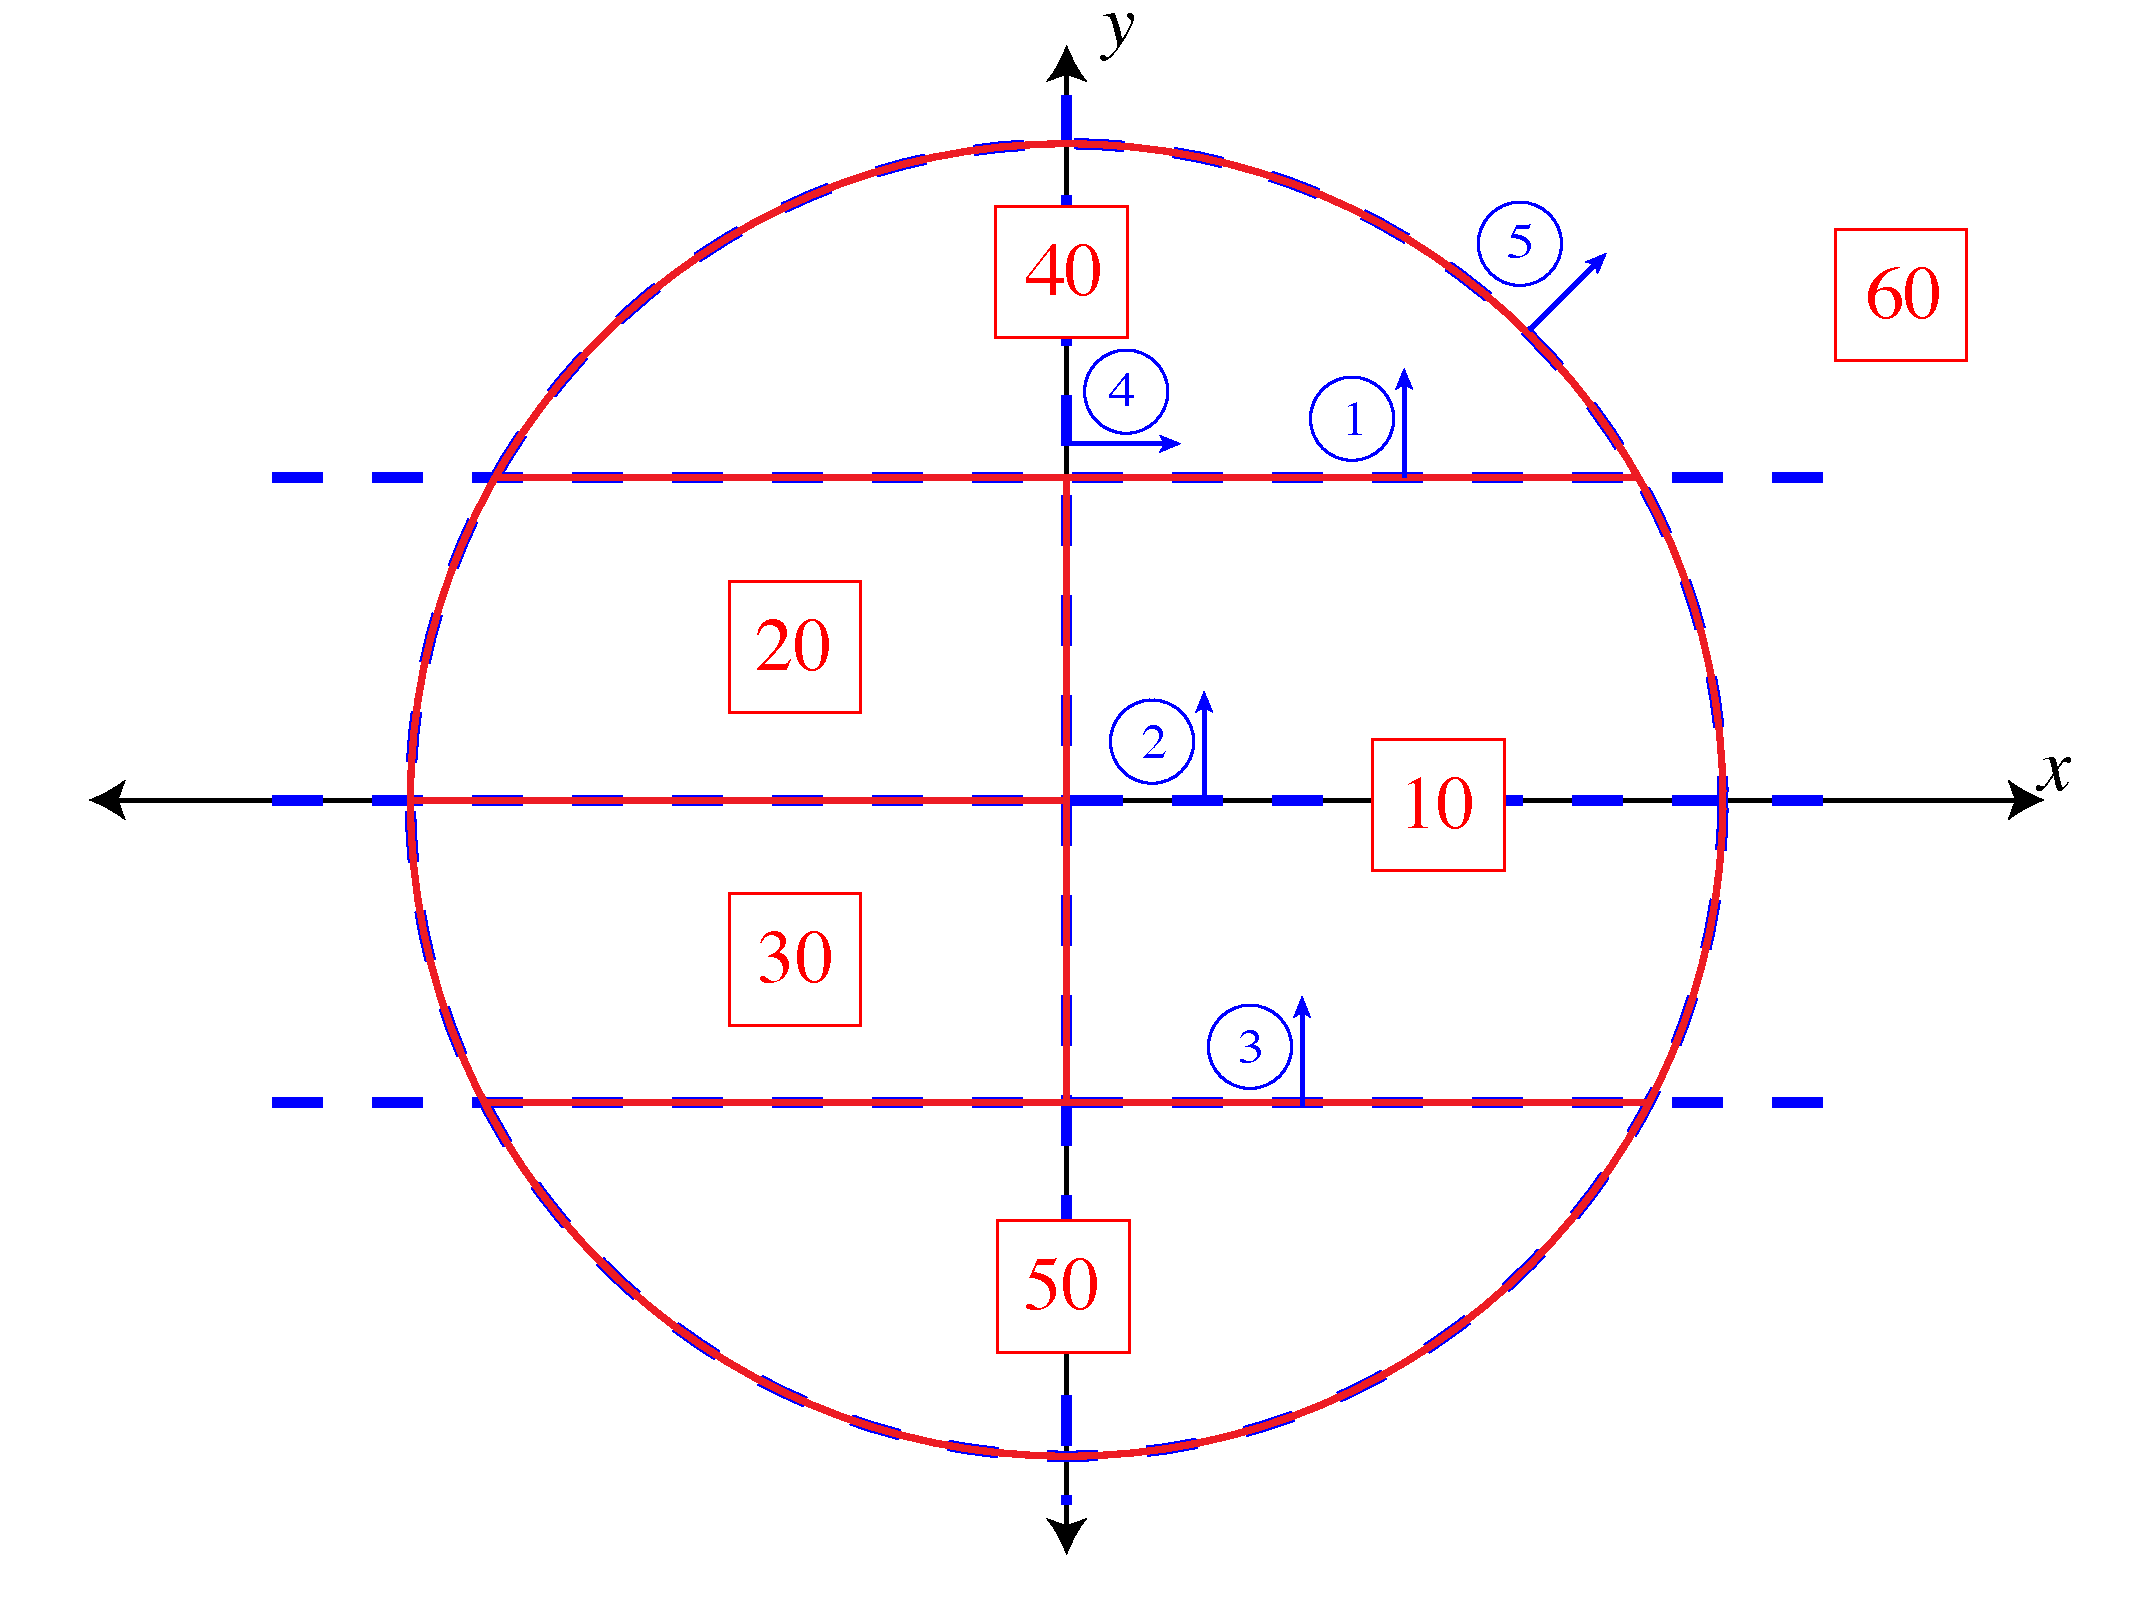
\includegraphics[width=\textwidth, keepaspectratio]{test_geom_1}
\end{columns}
\end{frame}

%%%%%%%%%%%%%%%%%%%%%%%%%%%%%%%%%%%%%%%%
\begin{frame}{Complex Geometry Description}
  \begin{center}
    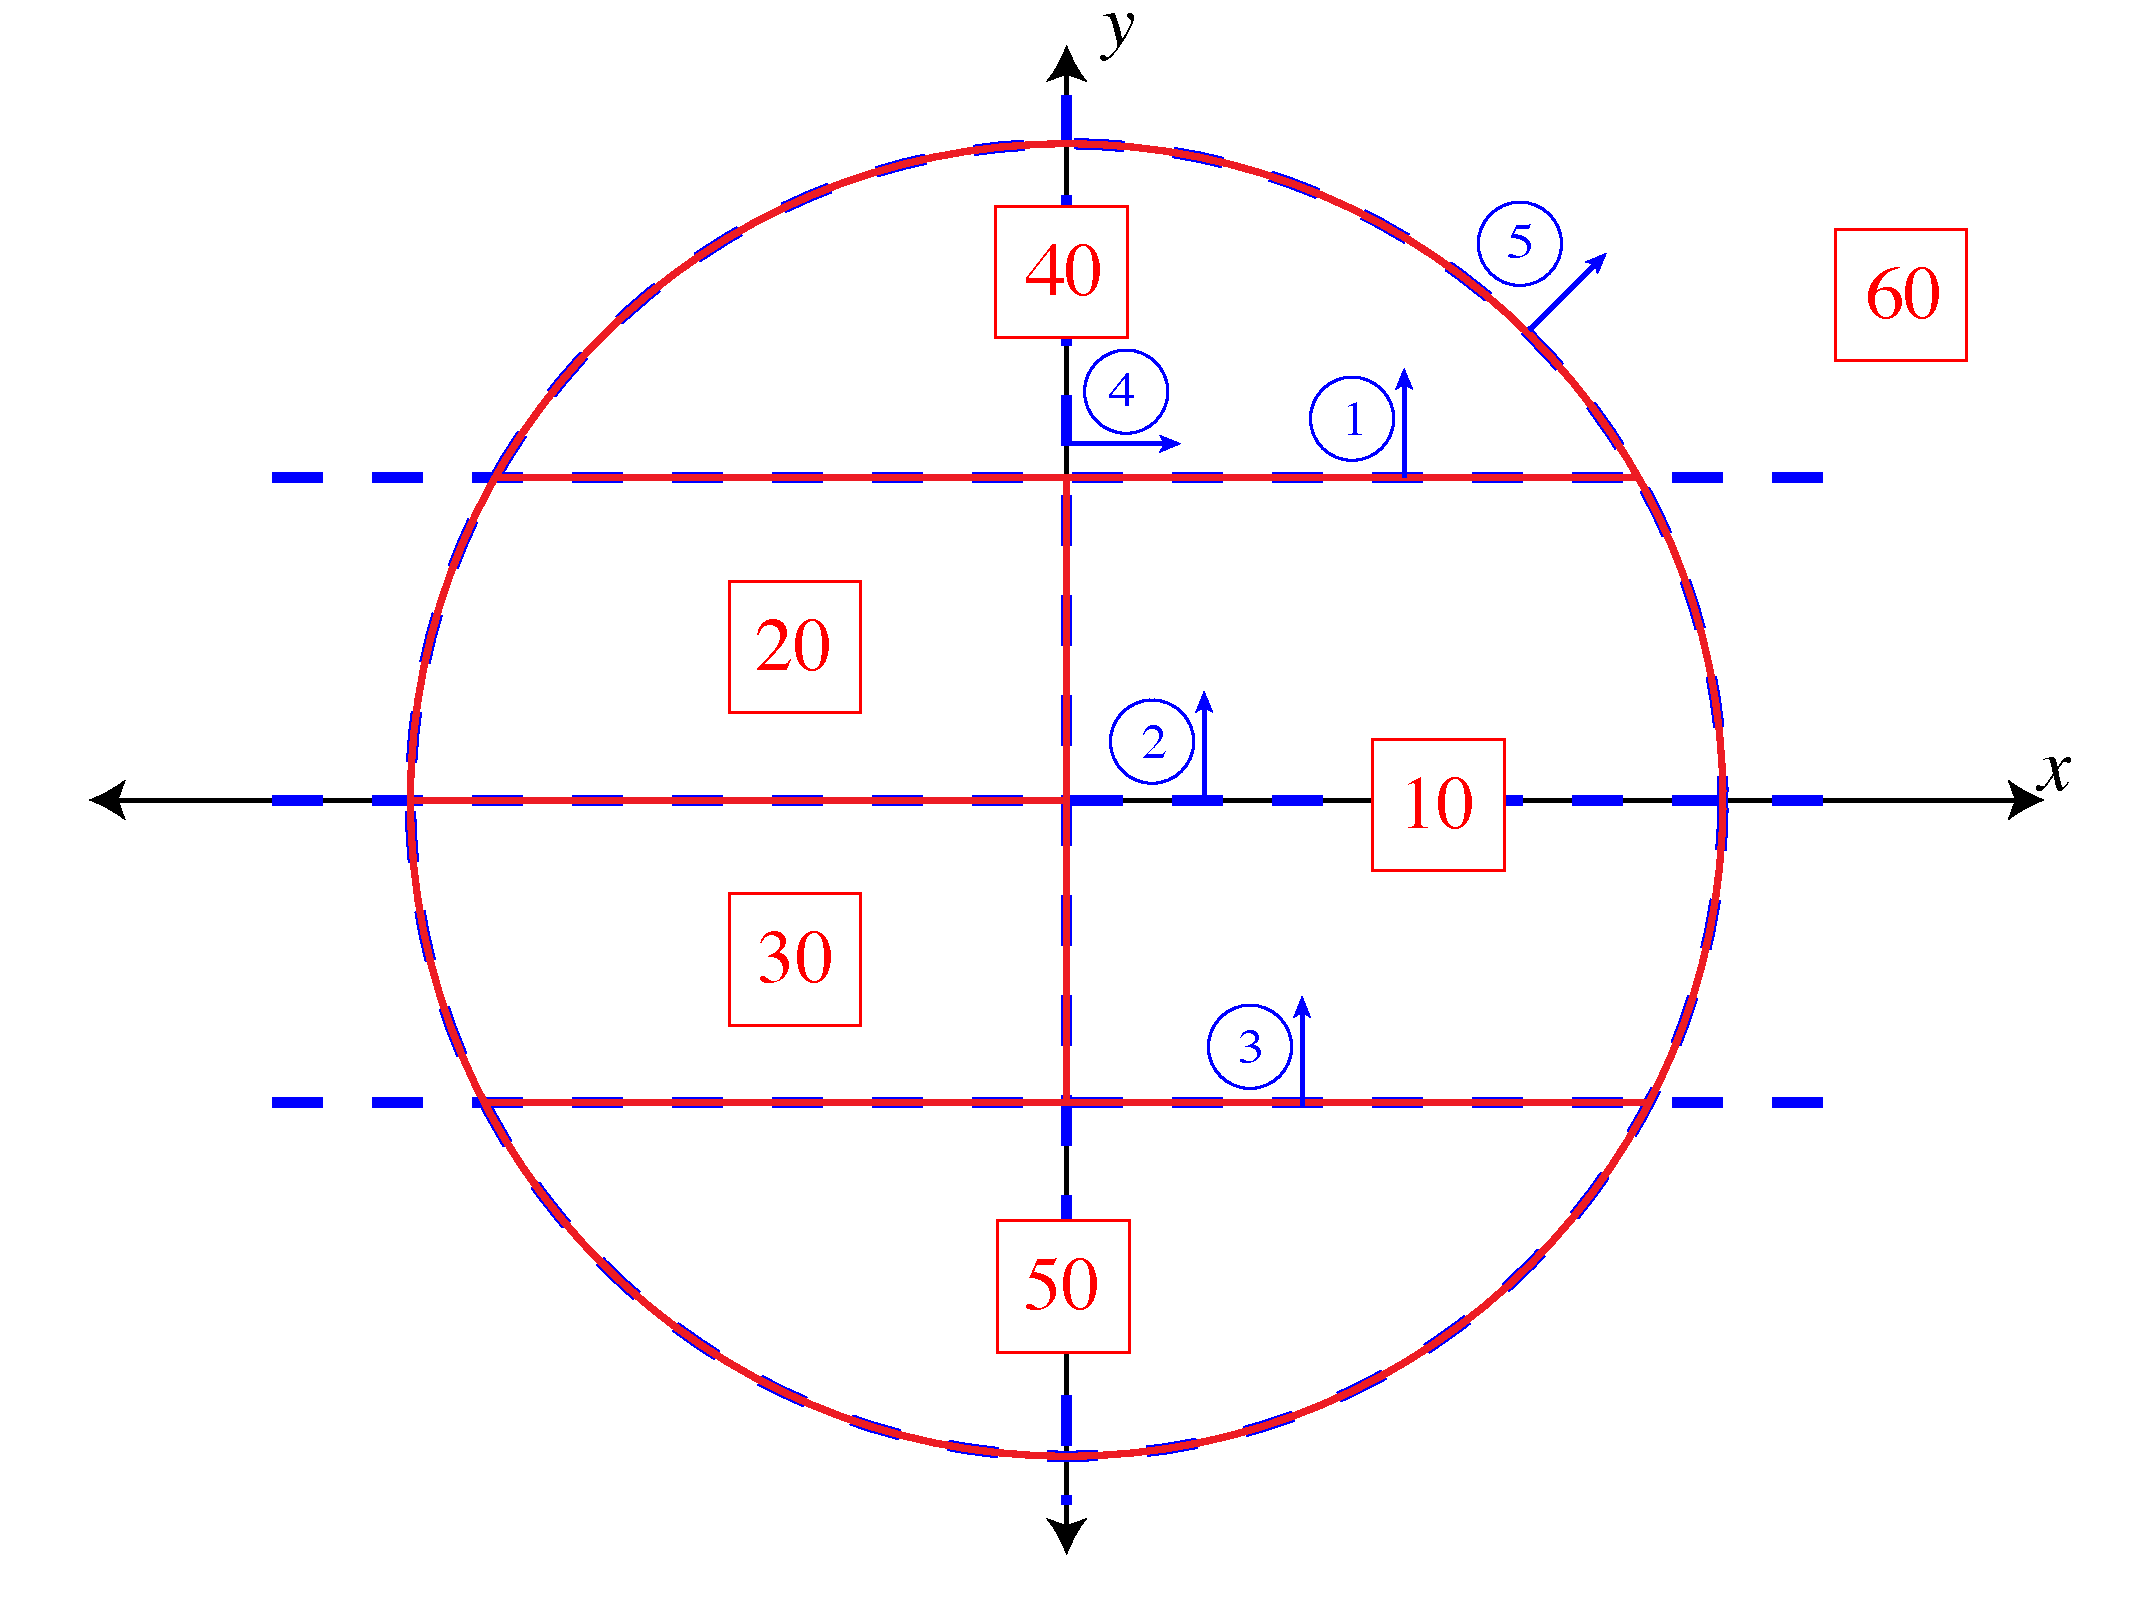
\includegraphics[width=0.9\textwidth, keepaspectratio]{test_geom_1}
  \end{center}
\end{frame}

%%%%%%%%%%%%%%%%%%%%%%%%%%%%%%%%%%%%%%%%
\begin{frame}[fragile]
\frametitle{Complex Geometry Output}
\fvset{fontsize=\tiny}%

\begin{Verbatim}
SURFACES: 
 SURFACE 5: [ SPHERE Center:          <0,0,0> Radius:     3 ]
 SURFACE 1: [ PLANE  Point:           <0,1,0> Normal vector:          <0,1,0> ]
 SURFACE 2: [ PLANE  Point:           <0,0,0> Normal vector:          <0,1,0> ]
 SURFACE 3: [ PLANE  Point:           <0,-1,0> Normal vector:          <0,1,0> ]
 SURFACE 4: [ PLANE  Point:           <0,0,0> Normal vector:          <1,0,0> ]
CELLS: 
 CELL 10: -5 -1 +3 +4 
 CELL 20: -5 -1 +2 -4 
 CELL 30: -5 -2 +3 -4 
 CELL 40: -5 +1 
 CELL 50: -5 -3 
 CELL 60: -5  <NEGATED>
SURFACES TO CELLS: 
 -5: 10 20 30 40 50 
 +5: 60 
 -1: 10 20 
 +1: 40 
 -2: 30 
 +2: 20 
 -3: 50 
 +3: 10 30 
 -4: 20 30 
 +4: 10 
NEIGHBORHOOD CONNECTIVITY: 
 CELL 10: -5:{60 } -1:{40 } +3:{50 } +4:{30 20 } 
 CELL 20: -5:{60 } -1:{40 } +2:{30 } -4:{10 } 
 CELL 30: -5:{60 } -2:{20 } +3:{50 } -4:{10 } 
 CELL 40: -5:{60 } +1:{10 20 } 
 CELL 50: -5:{60 } -3:{30 10 } 
 CELL 60: -5:{50 30 10 20 40 } 
\end{Verbatim}
\end{frame}  

%%%%%%%%%%%%%%%%%%%%%%%%%%%%%%%%%%%%%%%%%%%%%%%%%%%%%%%%%%%%%%%%%%%%%%%%%%%%
\subsection{Robustness: Tricky geometries}
\begin{frame}{Tricky geometries}
\begin{columns}[c]
\column{0.5\textwidth}
\begin{itemize}
  \item Spheres tangent at a point, spheres tangent to cylinder and plane along
    circles
  \item Also: transporting through corners
  \item Can we handle geometries with crazy intersections without losing
    particles?
\end{itemize}

\column{0.5\textwidth}
    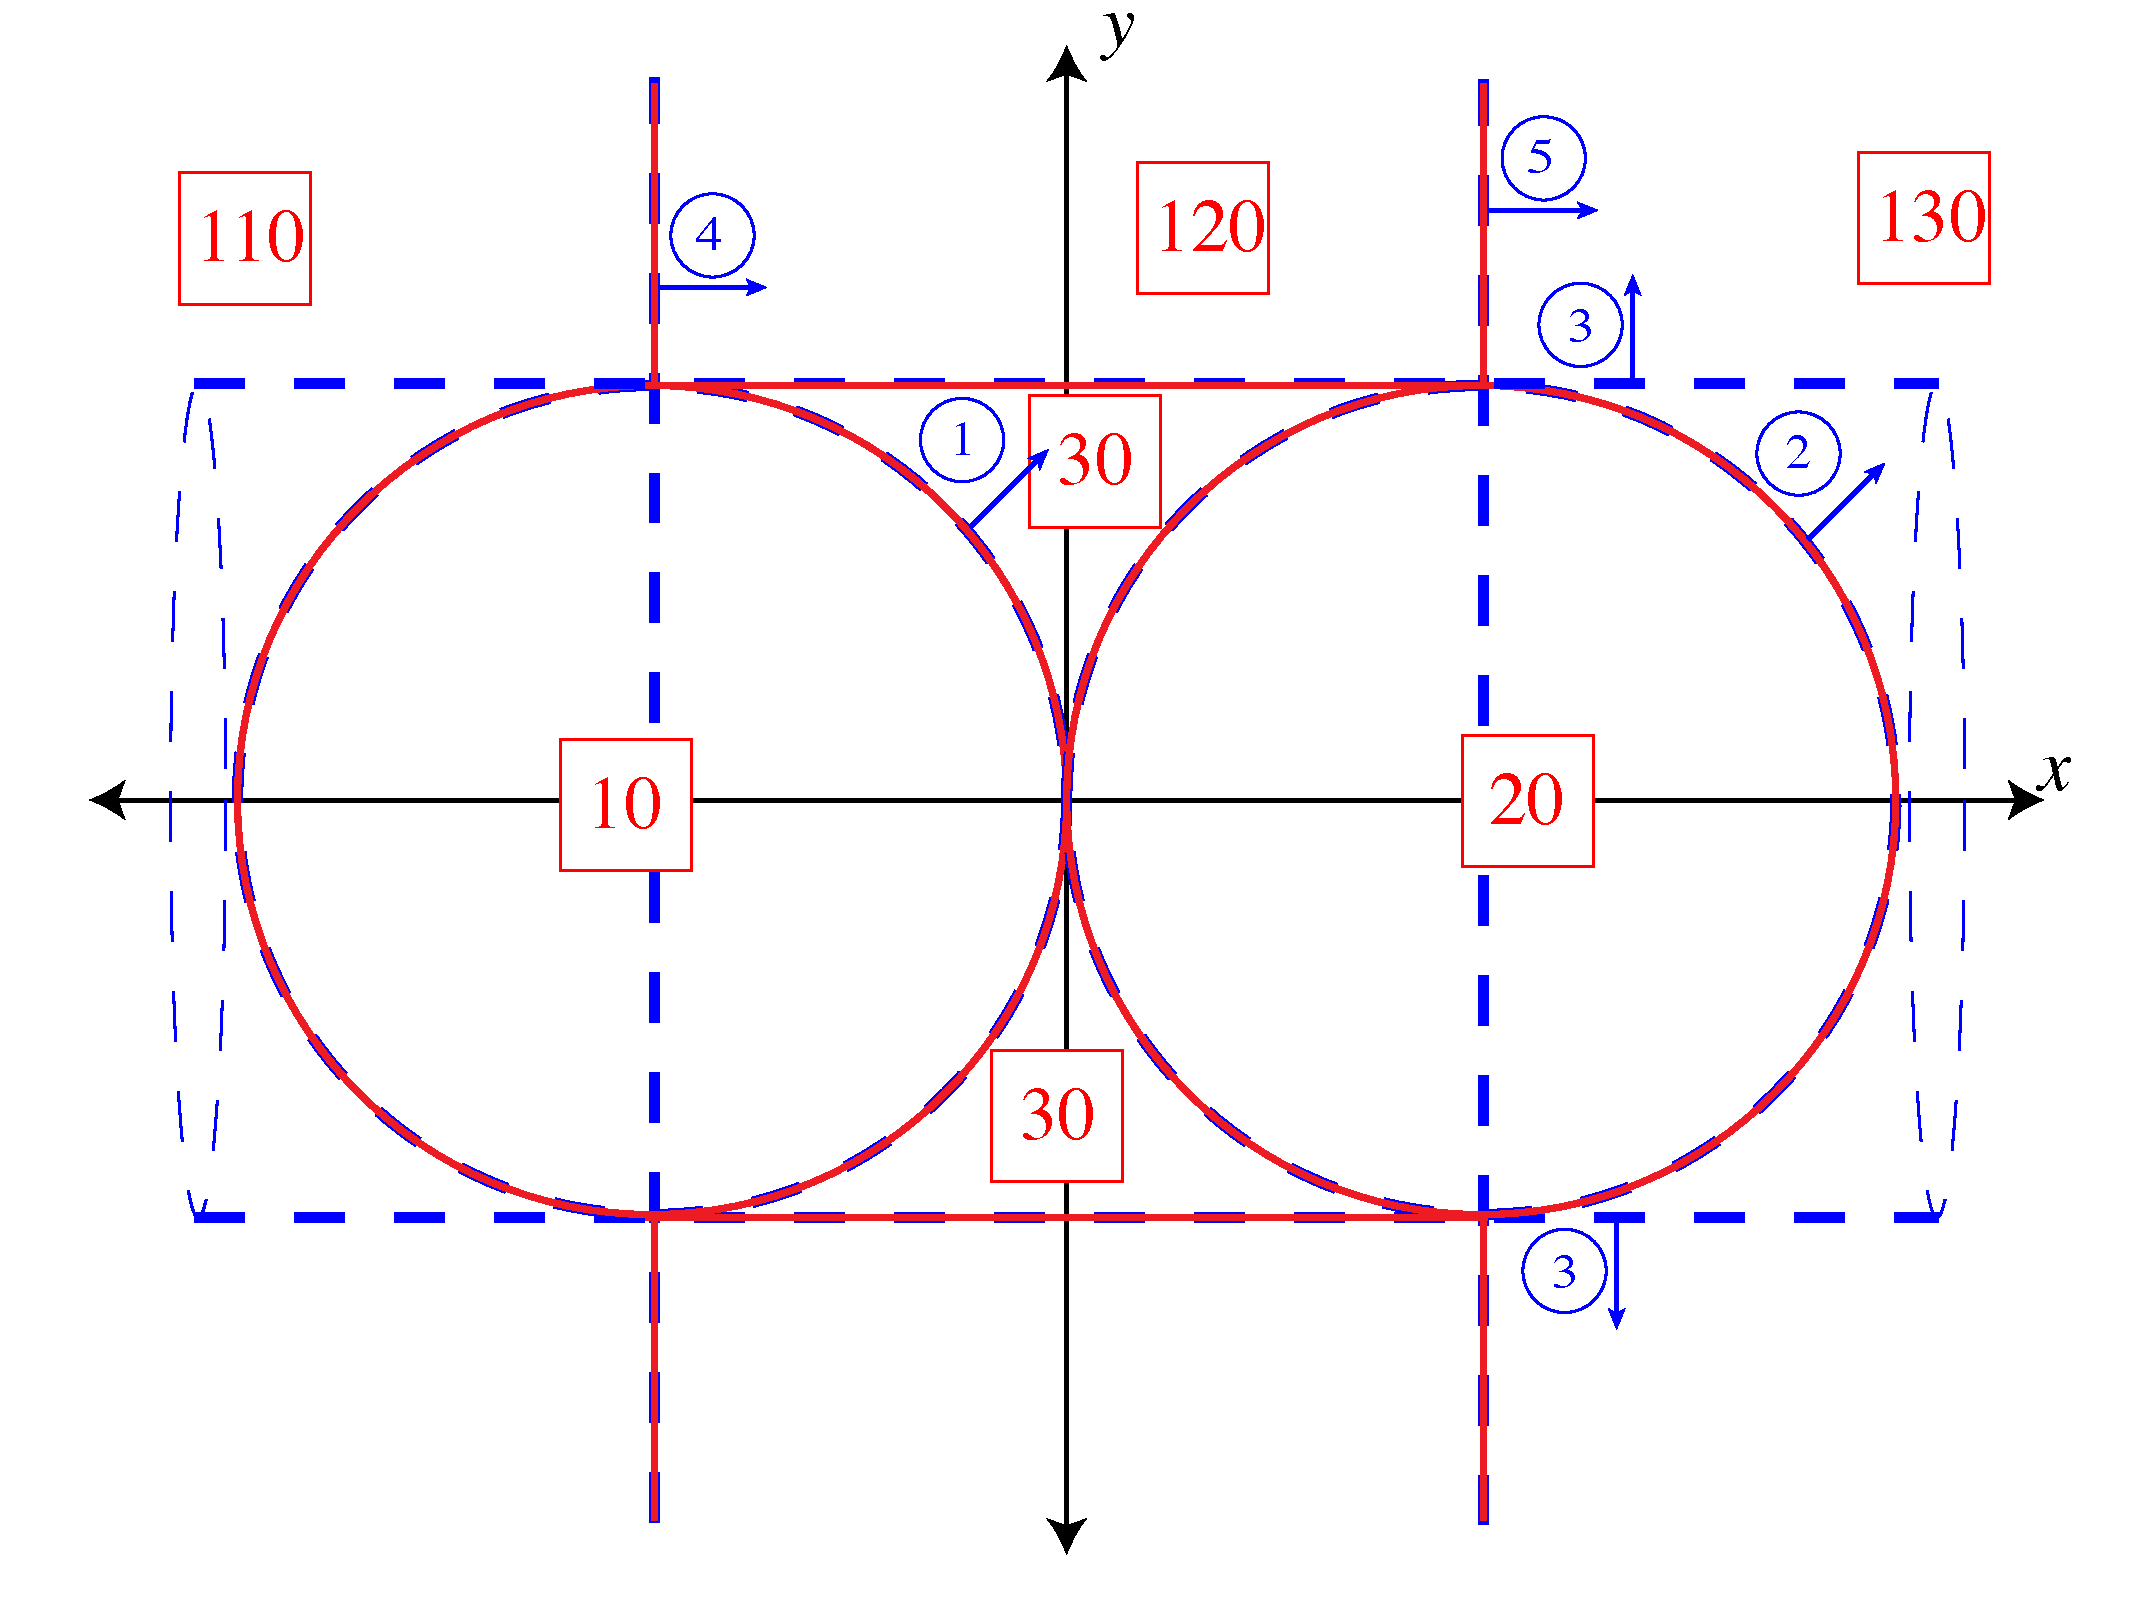
\includegraphics[width=\textwidth, keepaspectratio]{tricky_geometry}
\end{columns}
\end{frame}
%%%%%%%%%%%%%%%%%%%%%%%%%%%%%%%%%%%%%%%%
\begin{frame}{Yes, yes we can.}
    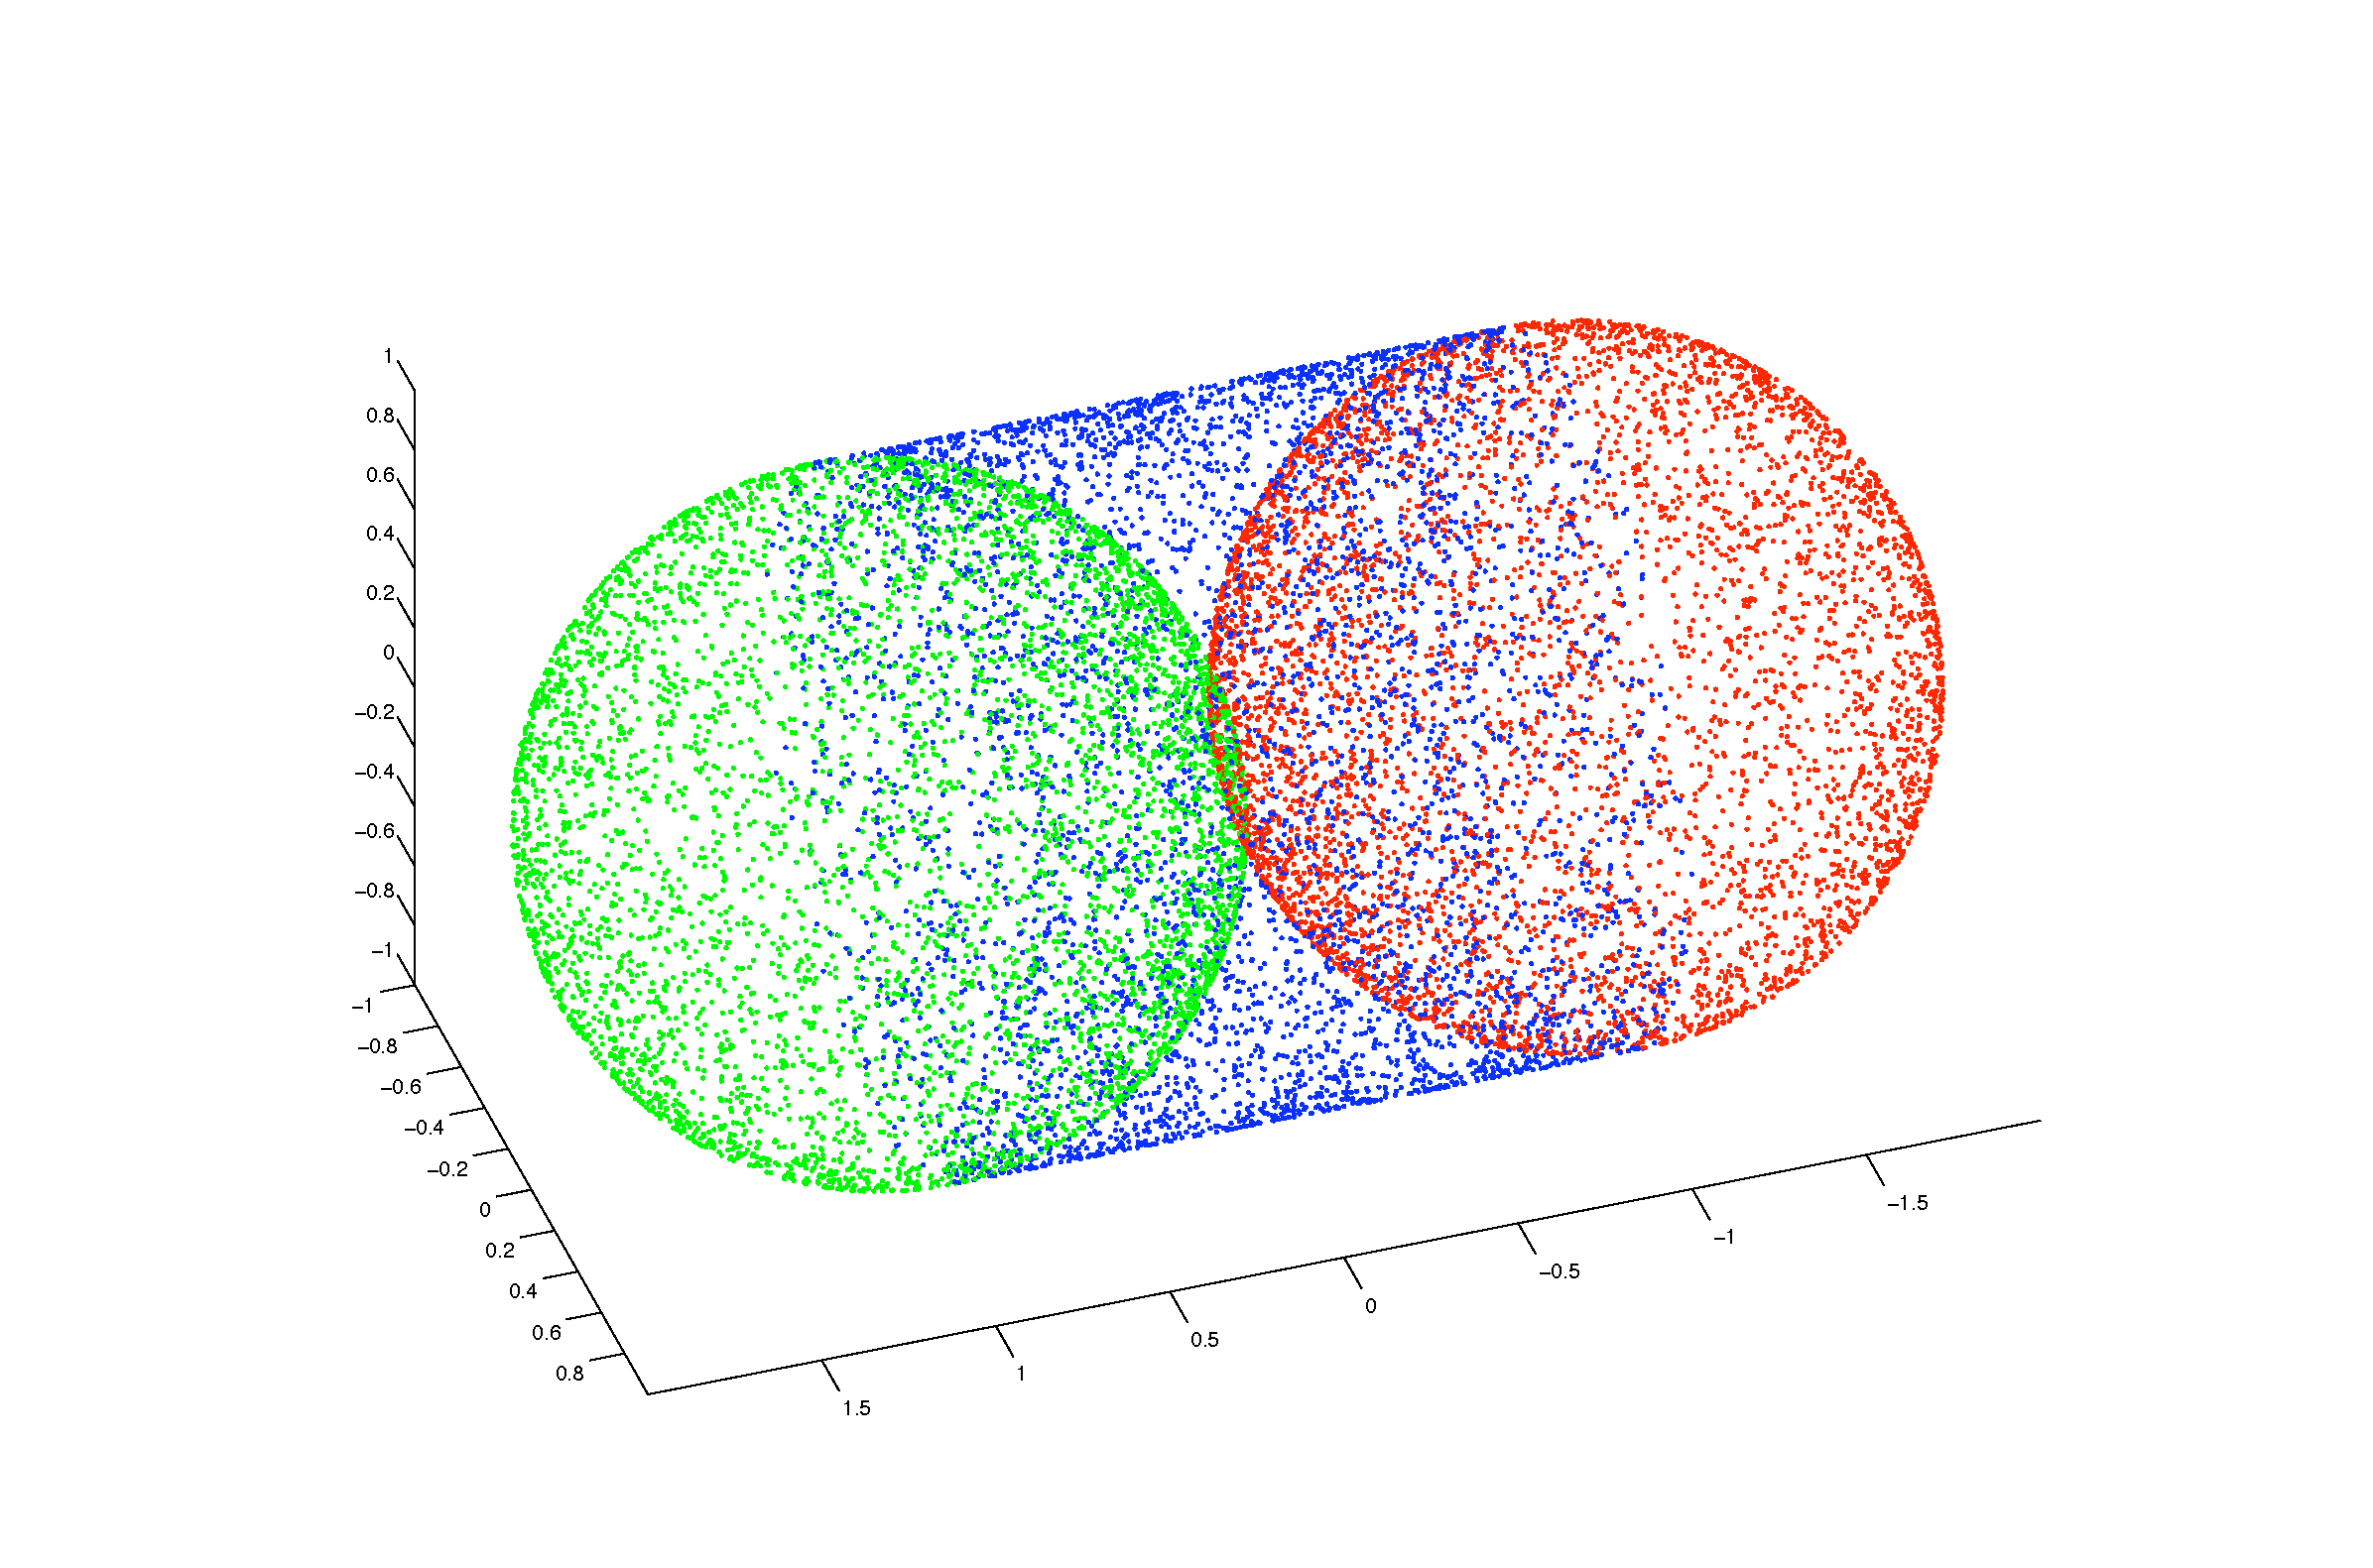
\includegraphics[width=\textwidth, keepaspectratio]{tricky_geometry_matlab}
\end{frame}
%%%%%%%%%%%%%%%%%%%%%%%%%%%%%%%%%%%%%%%%%%%%%%%%%%%%%%%%%%%%%%%%%%%%%%%%%%%%
\subsection{Speed: Mesh Geometry}
\begin{frame}
\frametitle{Mesh Geometry}
\begin{columns}[c]
\column{0.5\textwidth}
  \begin{itemize}
      \item Mesh has $N\times N \times N$ cells
      \item Checkerboard pattern of alternating total cross sections
          \begin{itemize}
              \item $\Sigma_t = 1.0$
              \item $\Sigma_t = 0.5$
          \end{itemize}
      \item Chose position at center of each cell
      \item Transport
      \begin{itemize}
          \item<2-> Forward Sweep
          \item<4-> Backward Sweep
          \end{itemize}
  \end{itemize}
%%%%%%%%%%%%%%%%%%%%%%%%%%%%%%%%%%%%%%%%
\column{0.5\textwidth}
  \only<1>{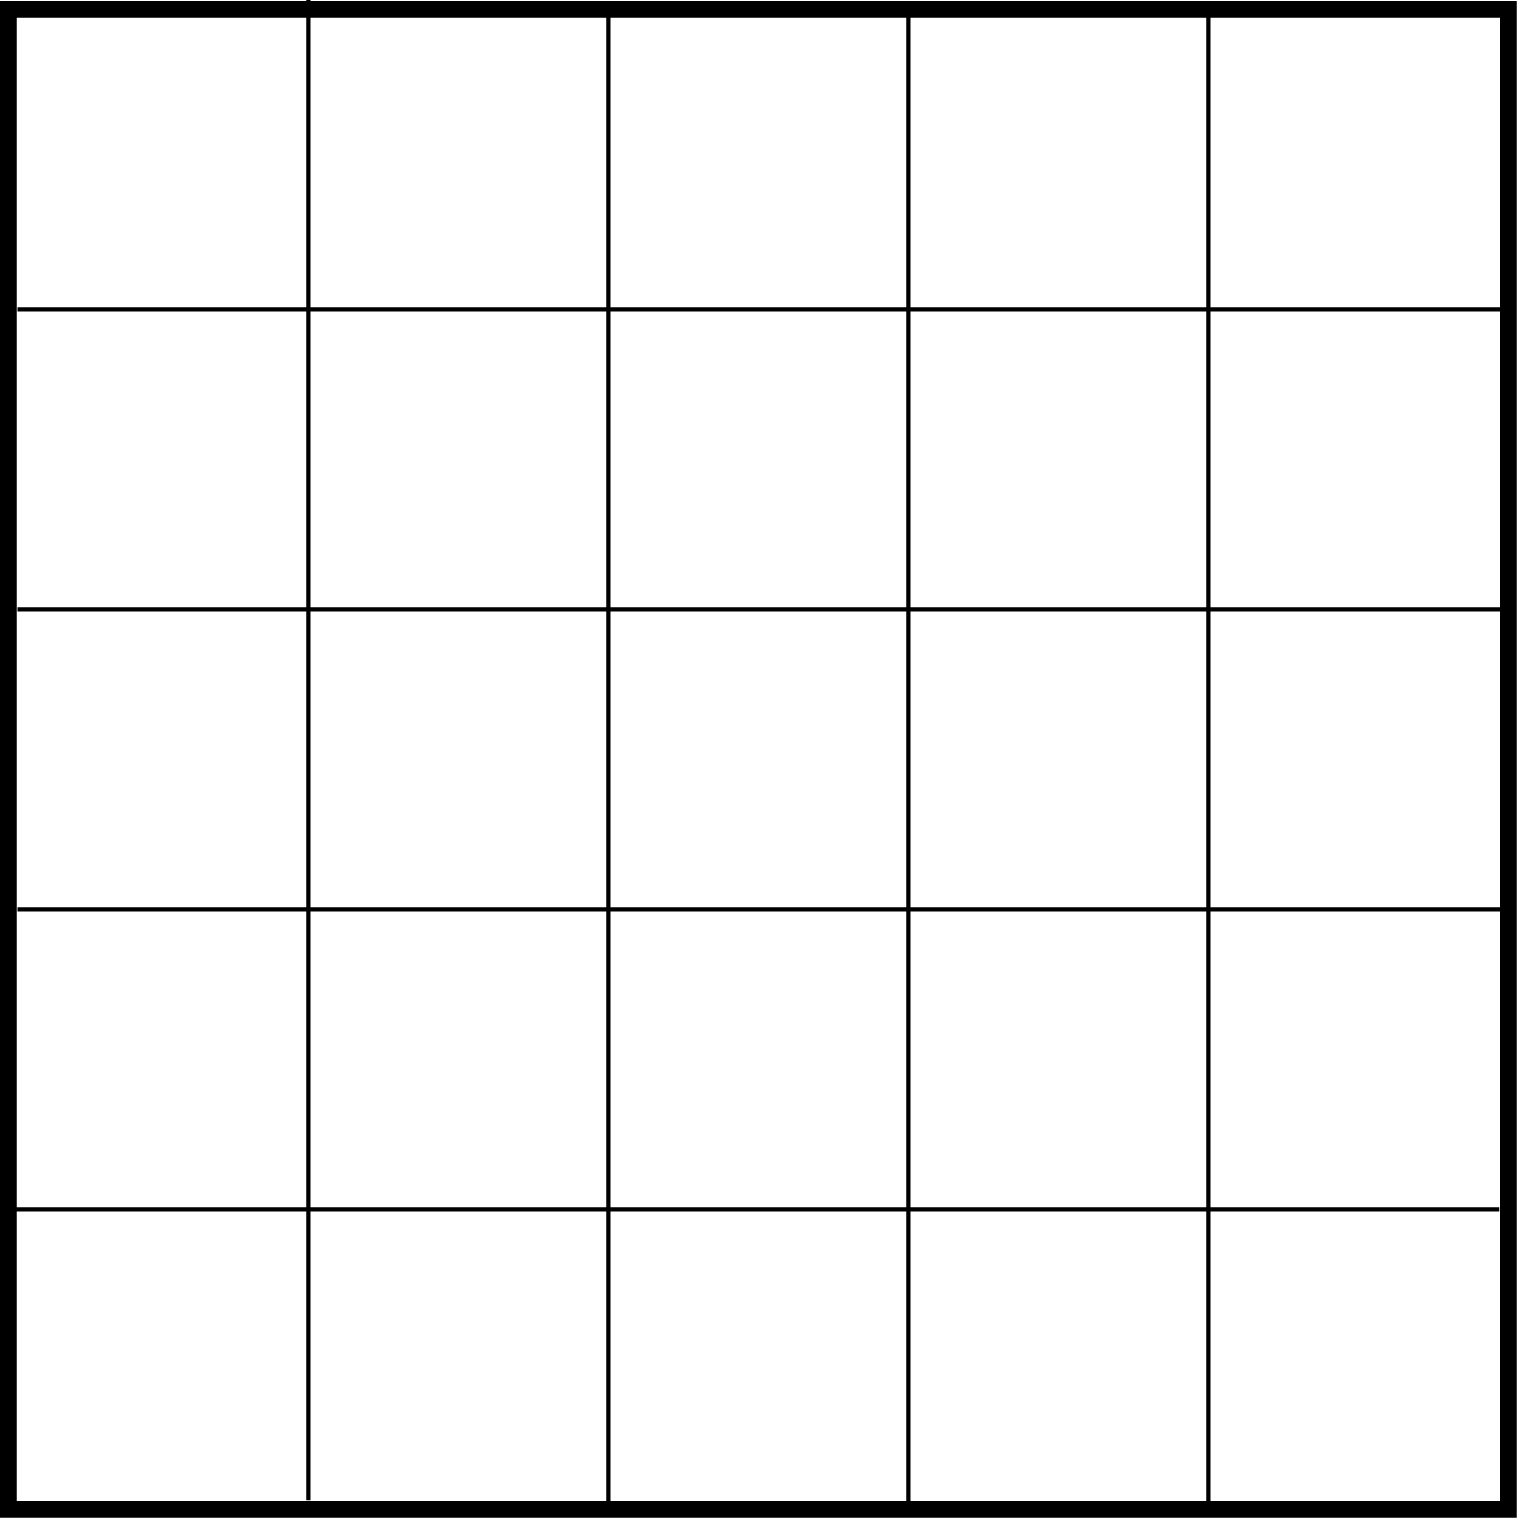
\includegraphics[width=\textwidth, keepaspectratio]{Mesh}}
  \only<2>{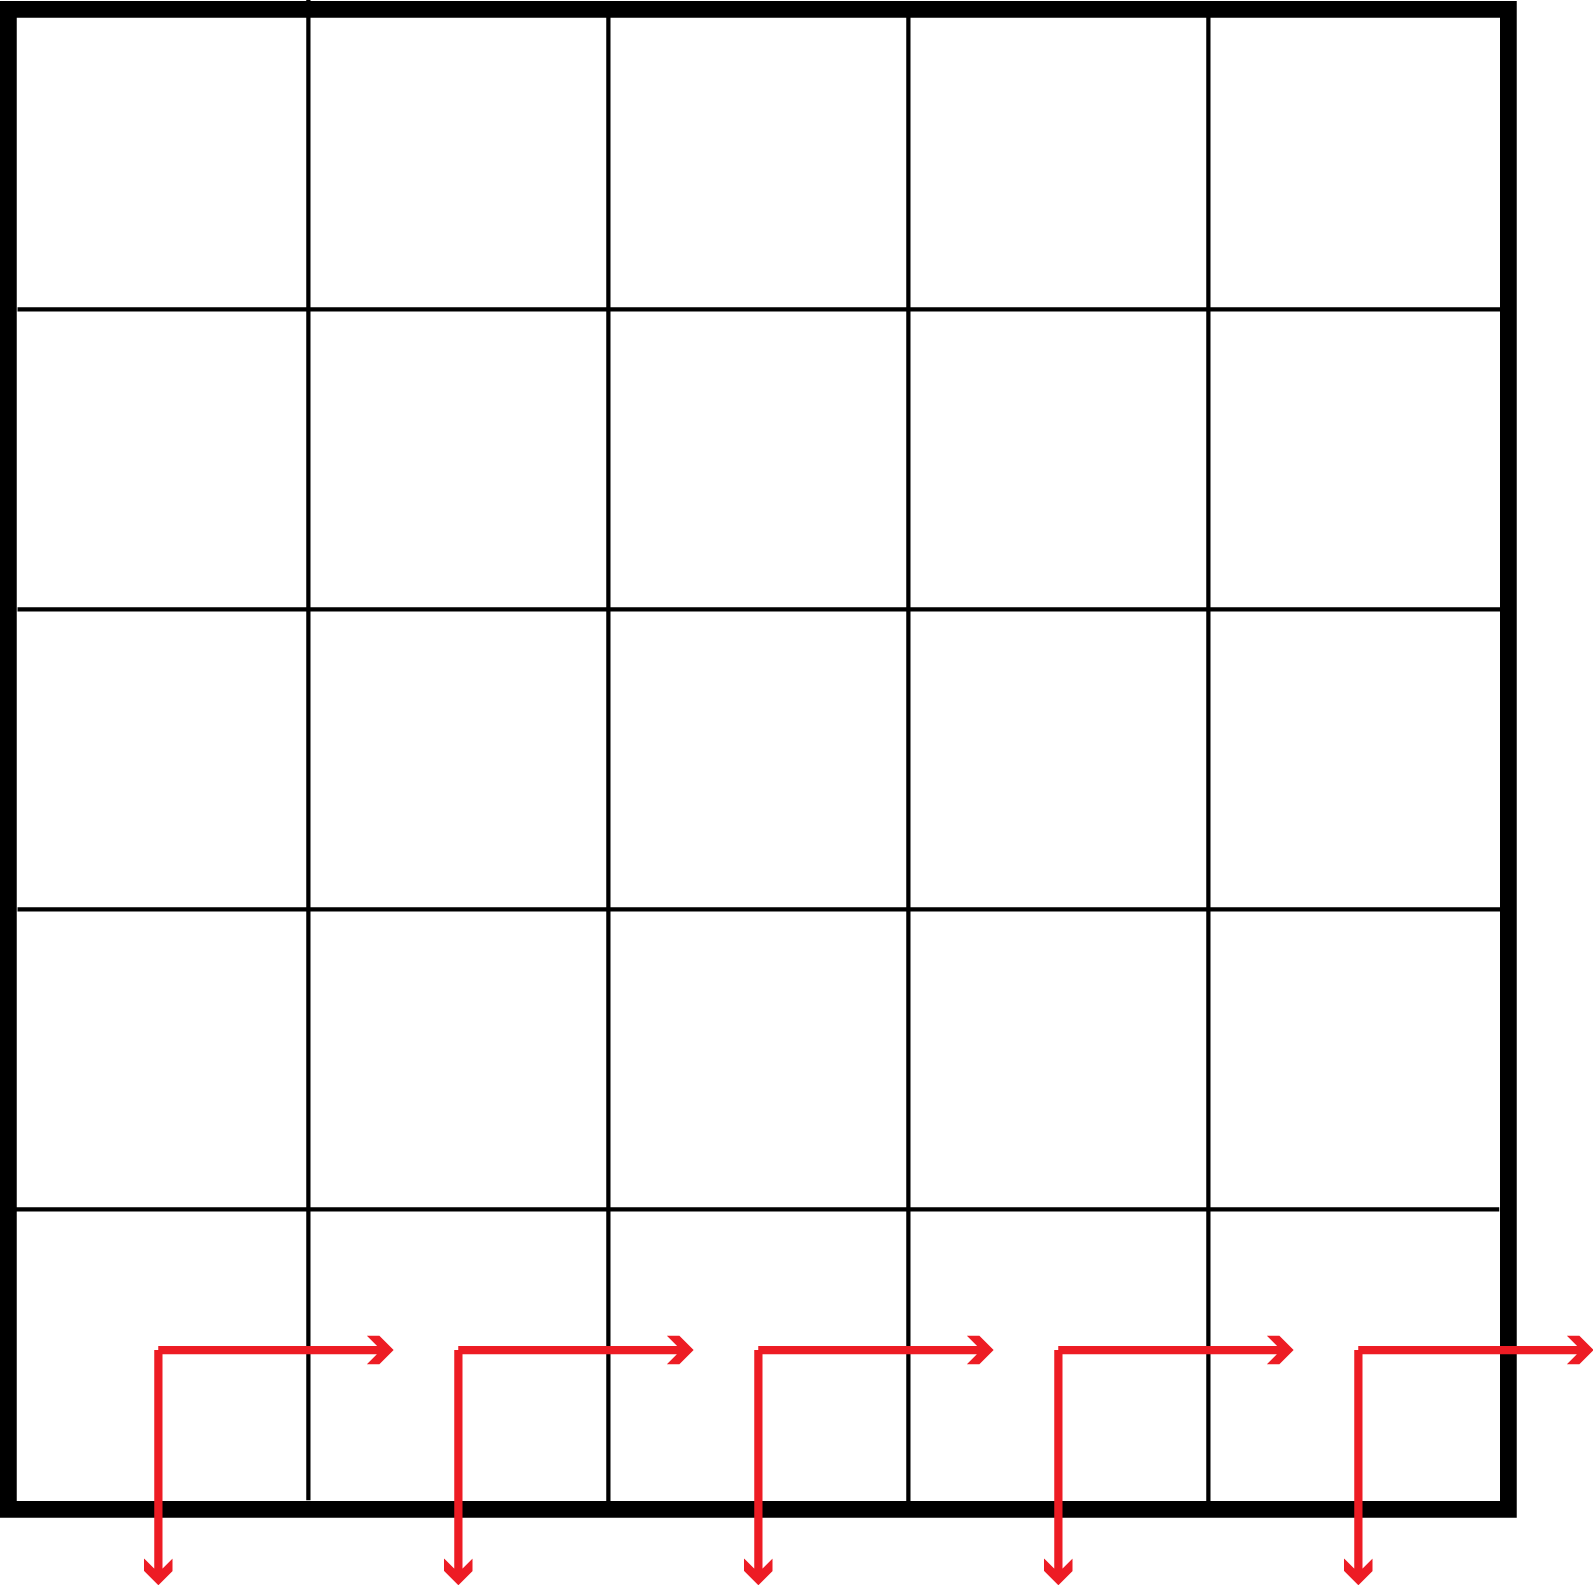
\includegraphics[width=\textwidth, keepaspectratio]{ForwardSweep}}
  \only<3>{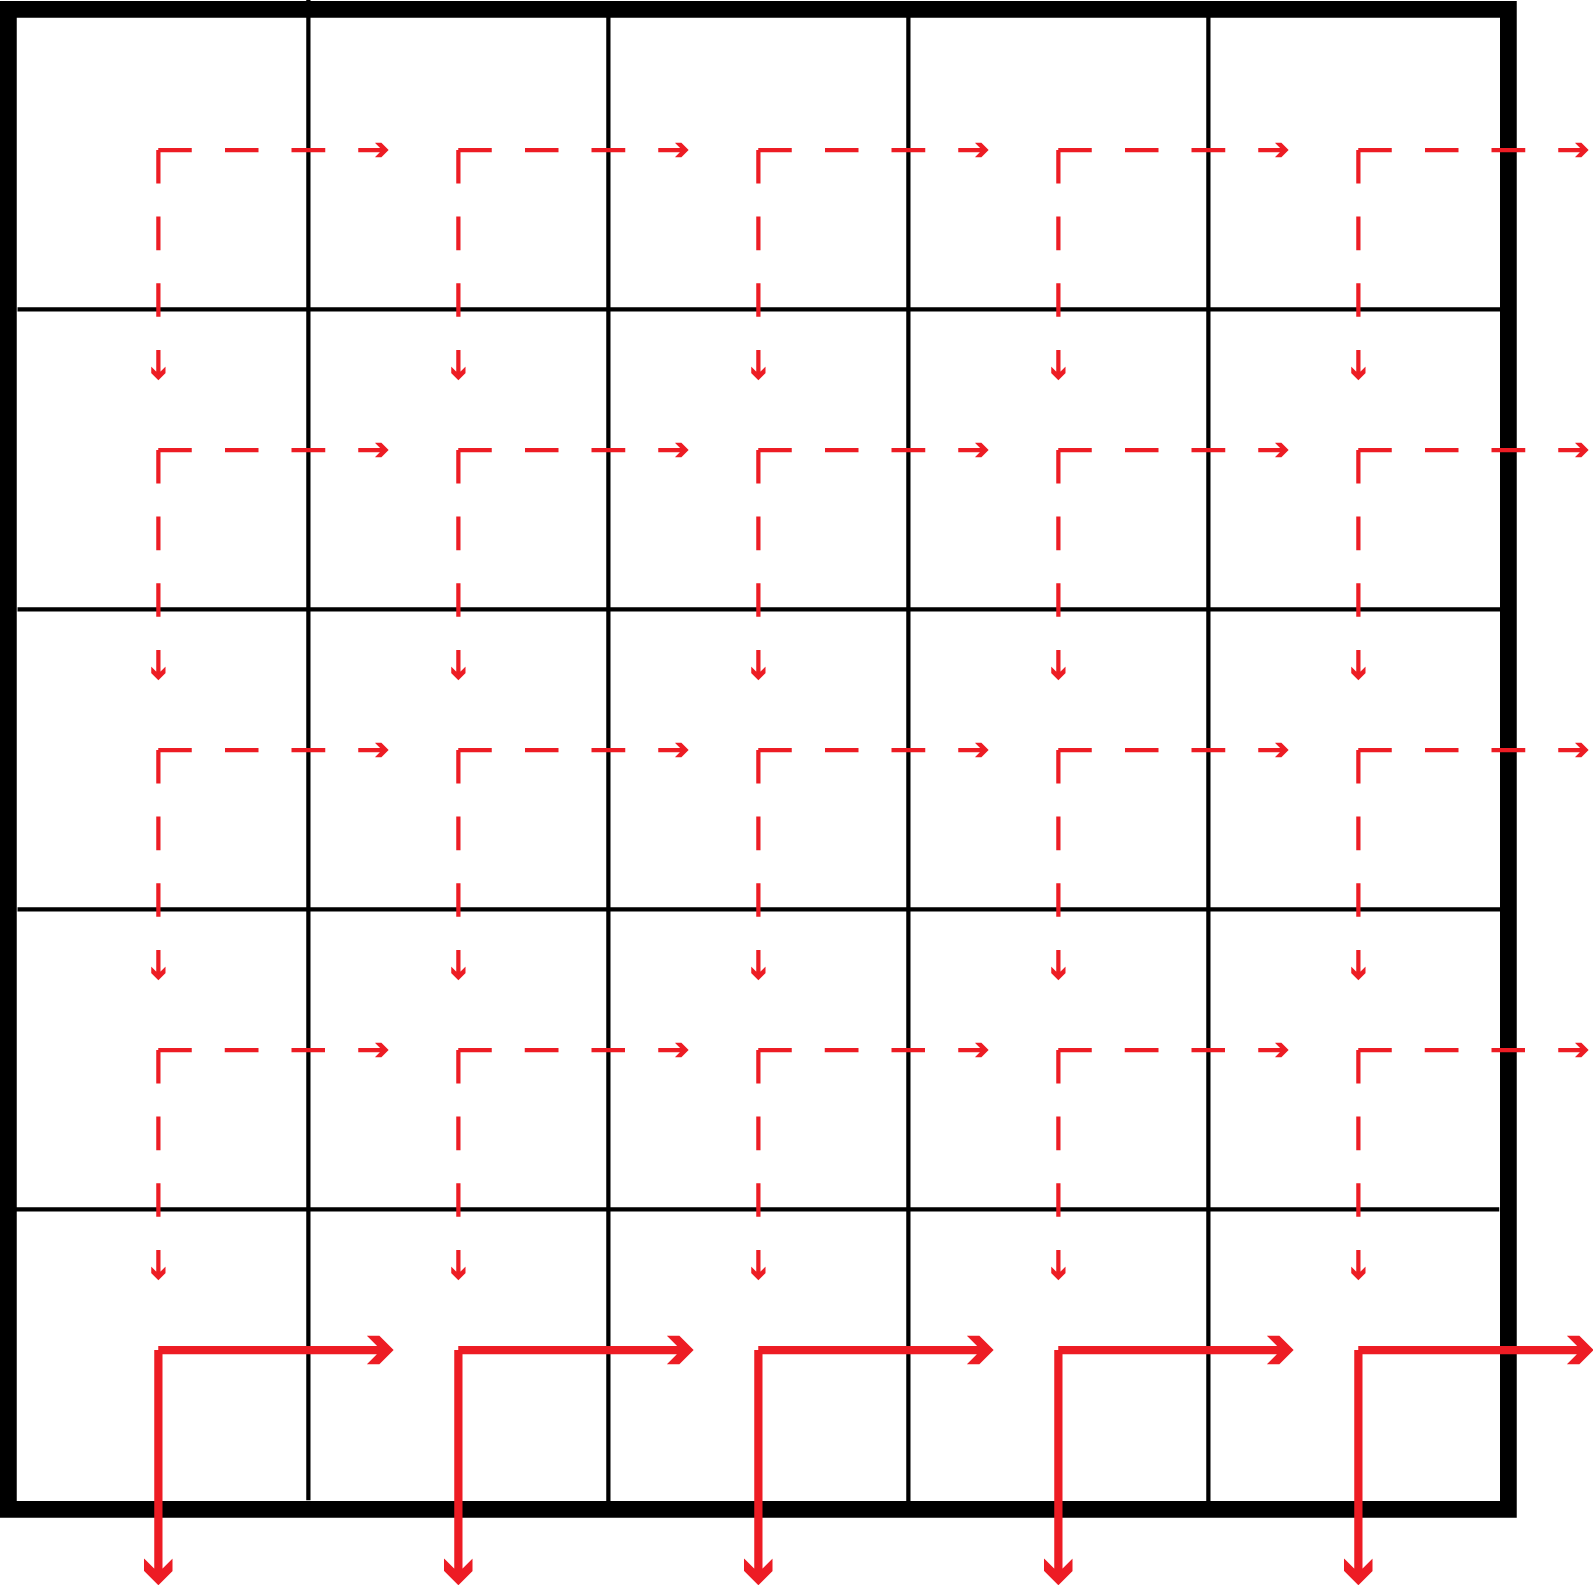
\includegraphics[width=\textwidth, keepaspectratio]{ForwardSweep-2}}
  \only<4>{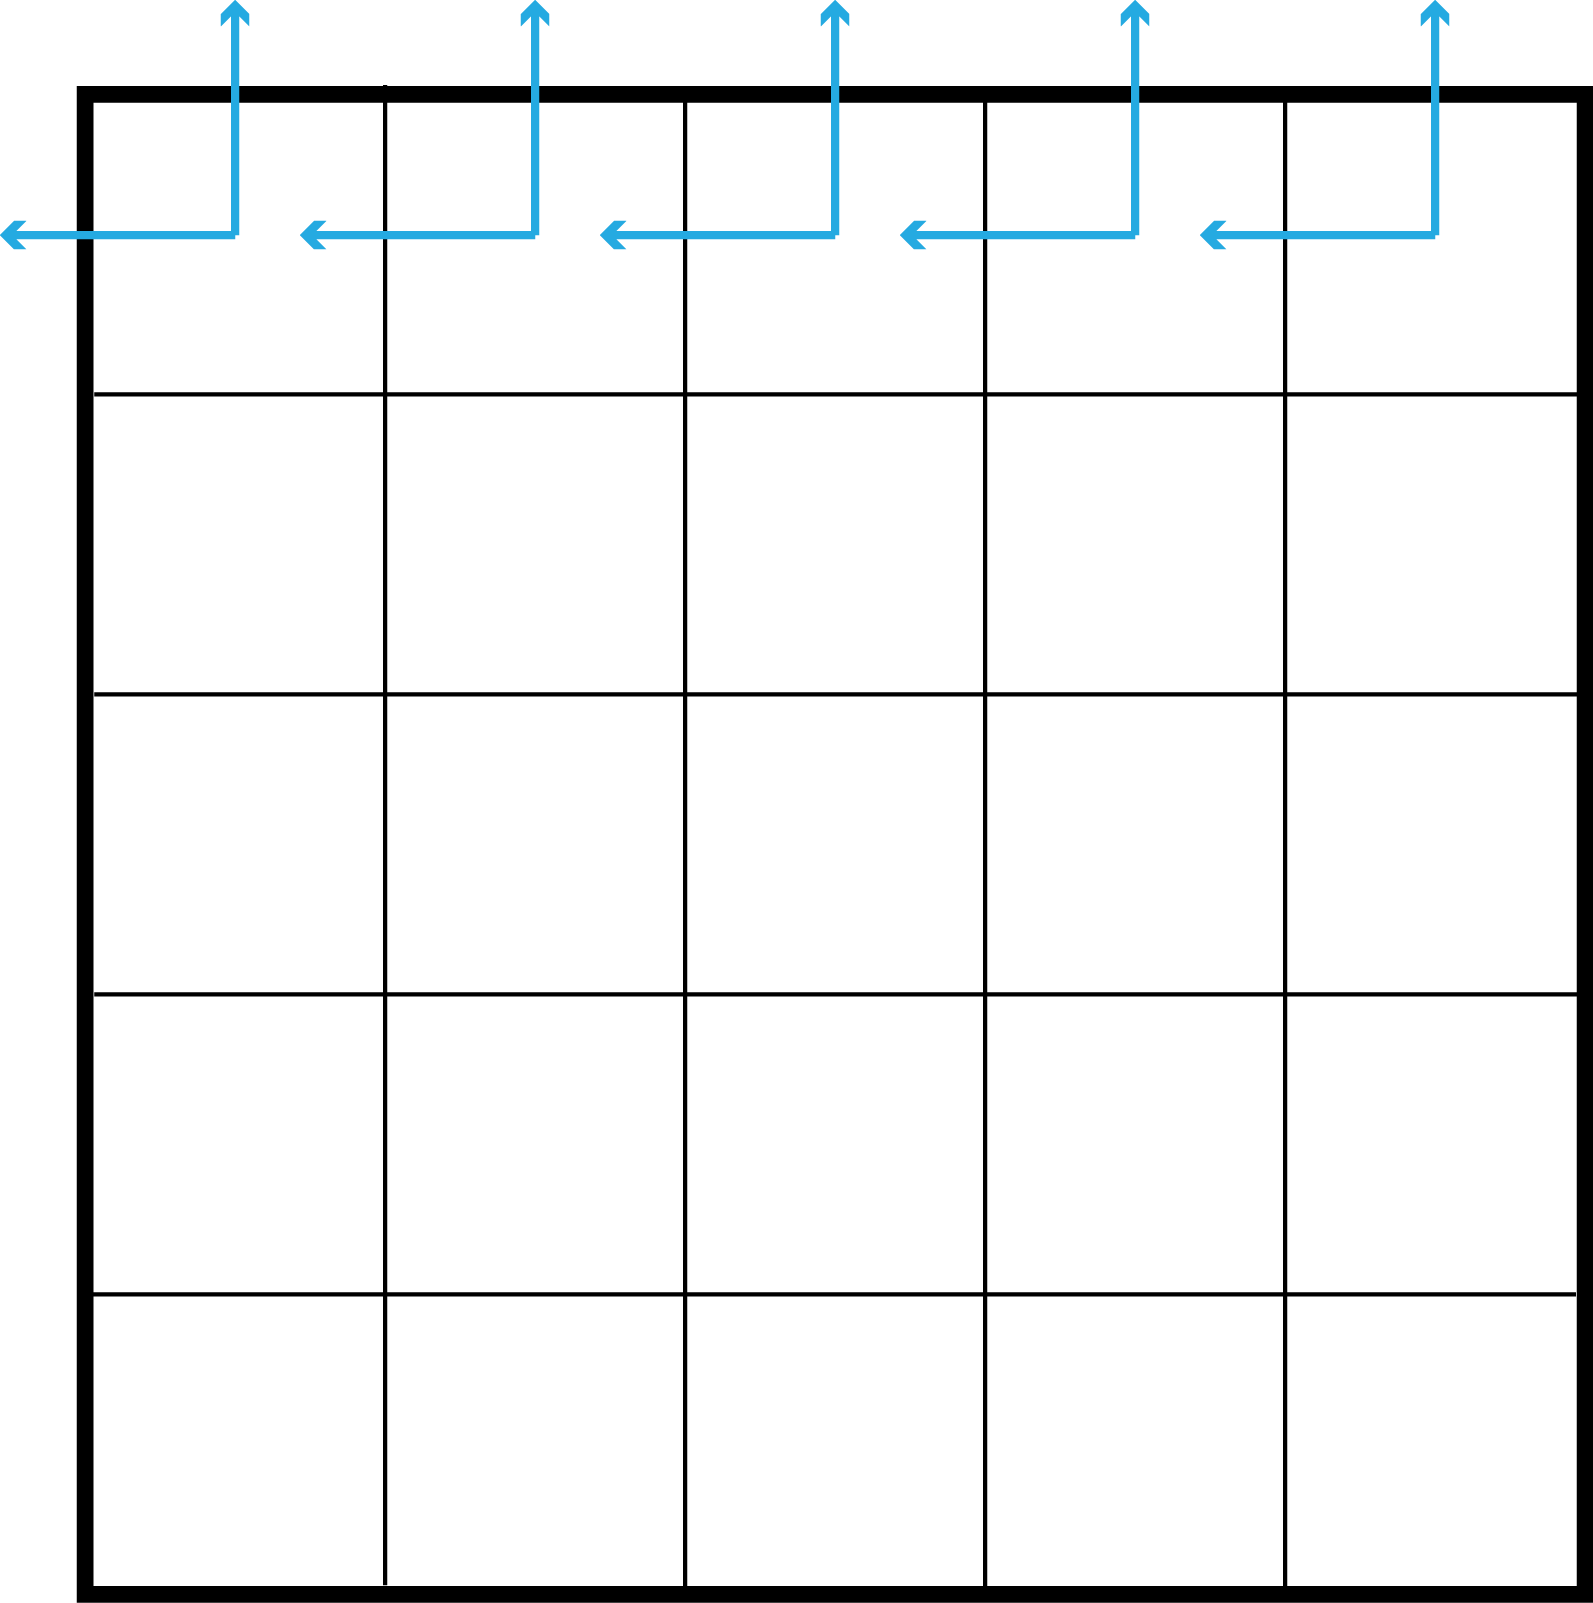
\includegraphics[width=\textwidth, keepaspectratio]{BackwardSweep}}
  \only<5>{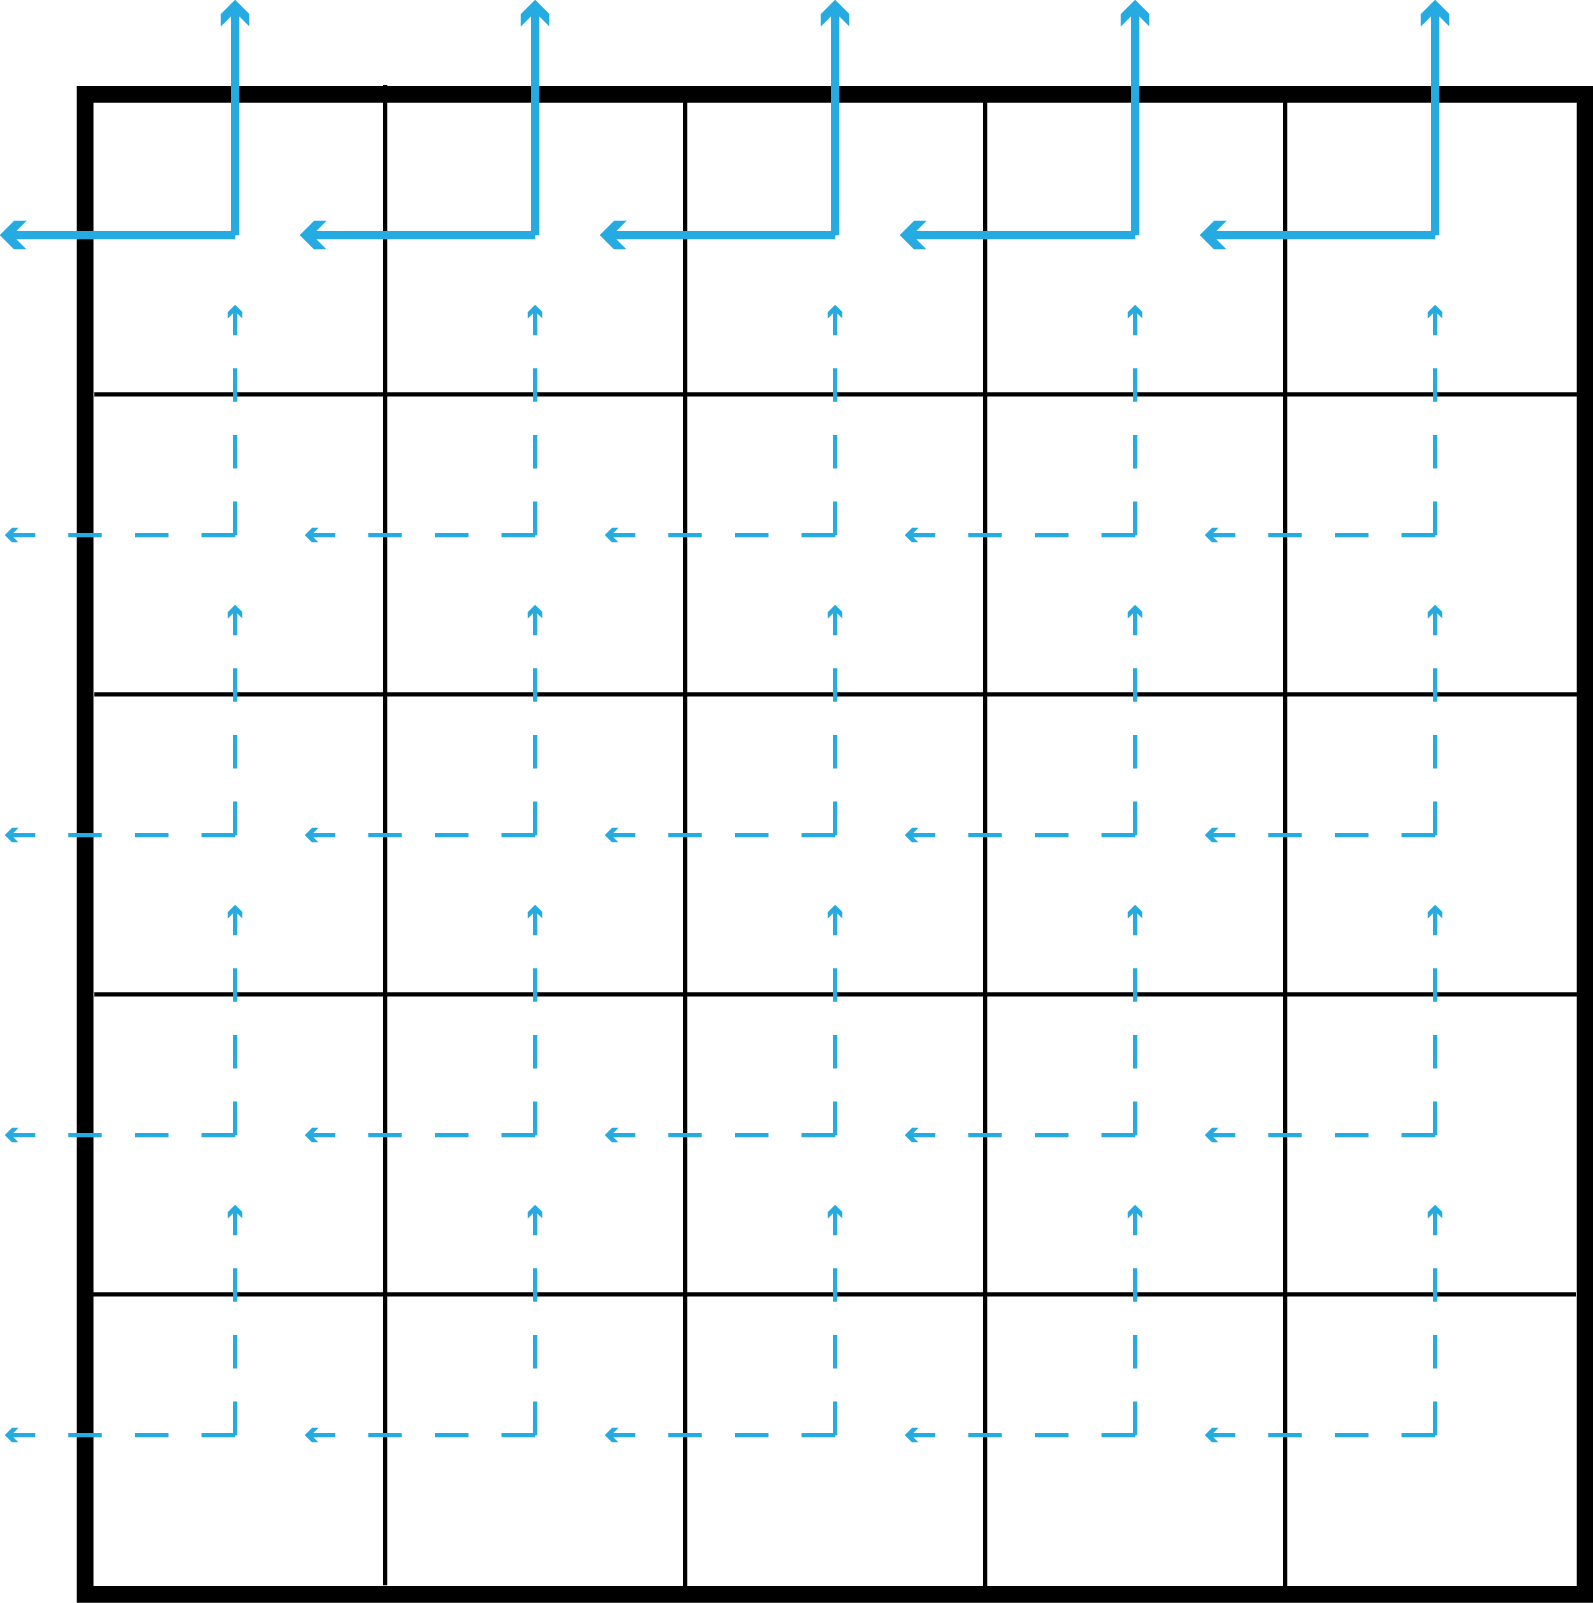
\includegraphics[width=\textwidth, keepaspectratio]{BackwardSweep-2}}
\end{columns}
\end{frame}
%%%%%%%%%%%%%%%%%%%%%%%%%%%%%%%%%%%%%%%%
\begin{frame}
    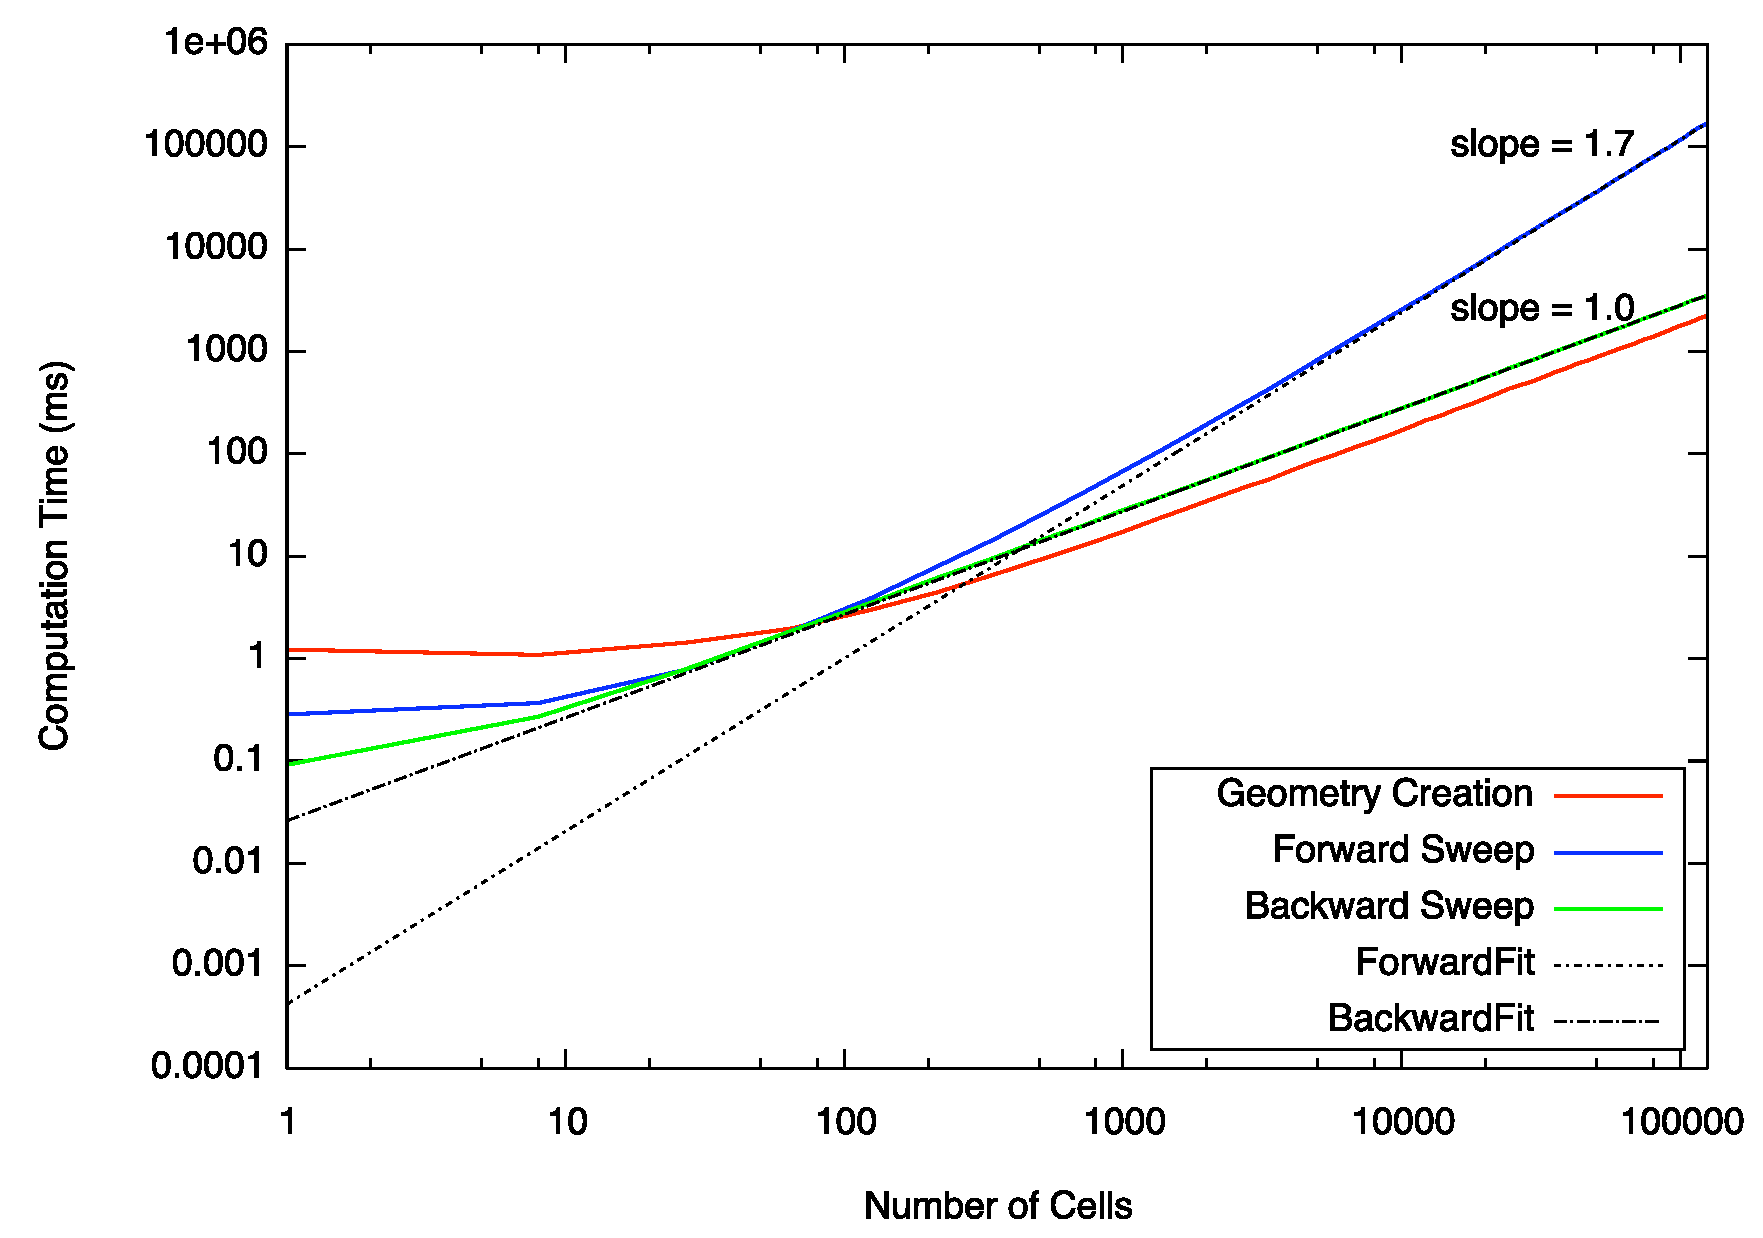
\includegraphics[width=\textwidth, keepaspectratio]{MeshTiming}
\end{frame}
%%%%%%%%%%%%%%%%%%%%%%%%%%%%%%%%%%%%%%%%
\begin{frame}
\begin{columns}[c]
\column{0.5\textwidth}
\begin{itemize}
    \item Mesh has $N\times N \times N$ cells
      \item Checkerboard pattern of alternating total cross sections
          \begin{itemize}
              \item $\Sigma_t = 1.0$
              \item $\Sigma_t = 0.5$
          \end{itemize}
    \item Random point picked
    \item Particle streams until it leaves geometry
\end{itemize}

\column{0.5\textwidth}
    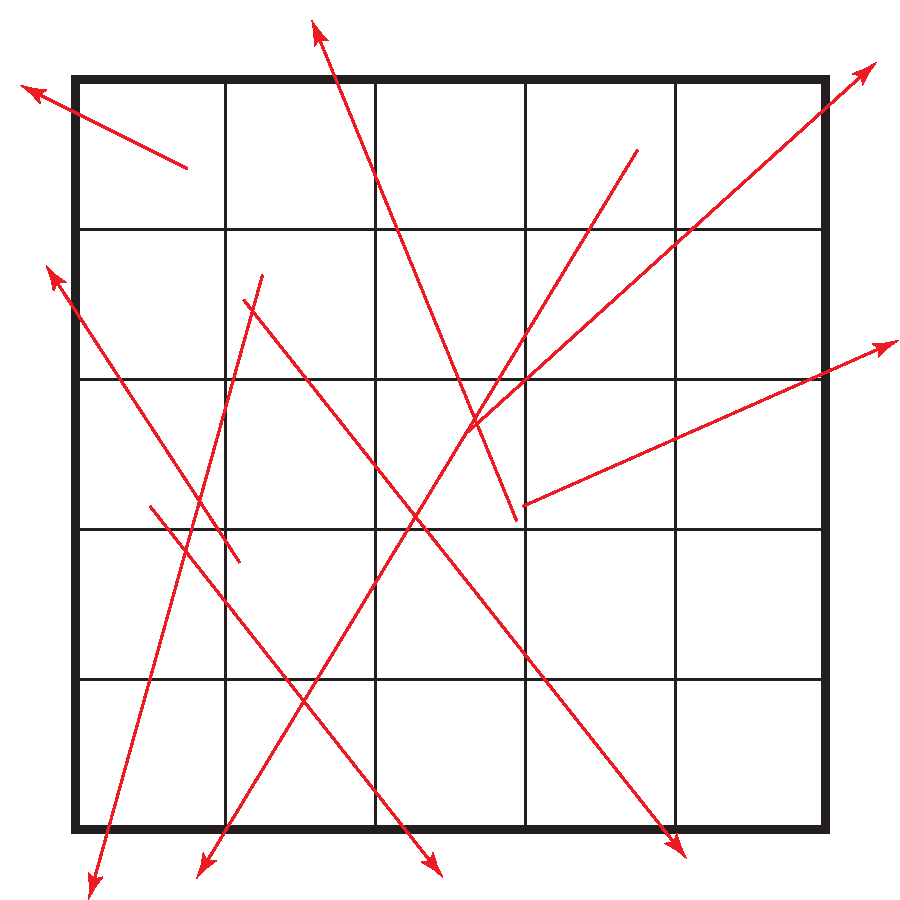
\includegraphics[width=\textwidth, keepaspectratio]{MeshCompGraphic}
\end{columns}
\end{frame}

%%%%%%%%%%%%%%%%%%%%%%%%%%%%%%%%%%%%%%%%
\begin{frame}
    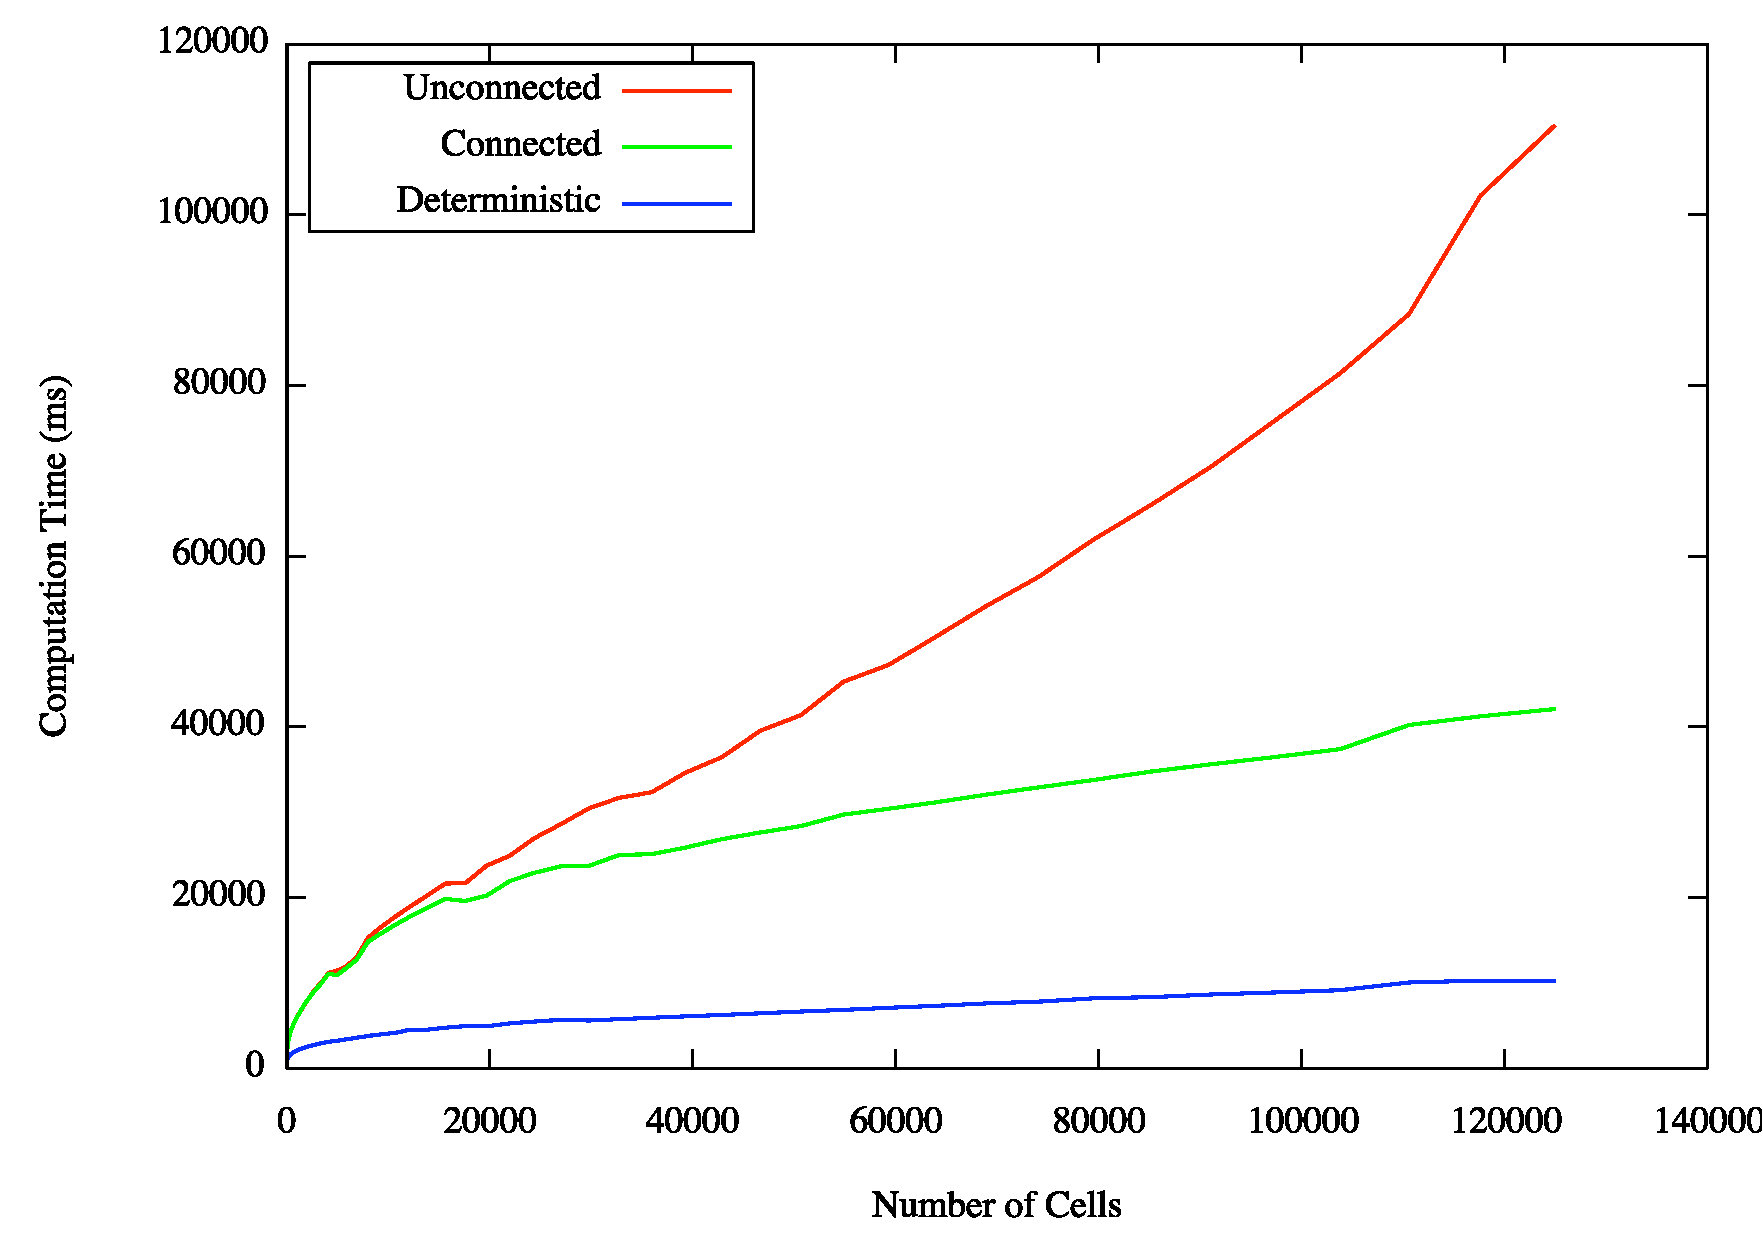
\includegraphics[width=\textwidth, keepaspectratio]{MeshComparison}
%    \includegraphics[width=\textwidth, keepaspectratio]{MeshComparison-2}
\end{frame}
%%%%%%%%%%%%%%%%%%%%%%%%%%%%%%%%%%%%%%%%%%%%%%%%%%%%%%%%%%%%%%%%%%%%%%%%%%%%
\section{Conclusions}

\begin{frame}
  \frametitle{Conclusions}
  \begin{itemize}
    \item<1-> Fully-functional combinatorial geometry
        \begin{itemize}
            \item Planes, Spheres, Cylinders
            \item Reflecting surfaces
            \item No lost particles
                \begin{itemize}
                    \item Complex and ``tricky'' geometry
                    \item Scale independent
                \end{itemize}
            \item Automatically generate connectivity
        \end{itemize}
    \item<2-> Caching connectivity improves runtime
   
    \item<3-> Combinatorial geometry concept is intuitive
    \item<4-> Implementation is difficult
        \begin{itemize}
            \item We implemented the geometry code in half a semester
            \item Available at \color{blue}{http://code.google.com/p/mcgeometry}
        \end{itemize}
     \item<5-> Better than doing the last homework assignment!
         \begin{itemize}
             \item Takes more time, but\dots
             \item Is more useful (to us) in the long run
         \end{itemize}
     \item<6-> \color{red}{We deserve an A+}
  \end{itemize}
\end{frame}

\begin{frame}
  \frametitle{Future work}
  \begin{itemize}
	 \item Write ``restart file'' for geometry (including connectivity)
   \item Use count of unmatched surfaces to obviate extra ``is point inside''
     checking of completed, simply connected geometries
   \item Further optimization tricks
  \end{itemize}
\end{frame}
%%%%%%%%%%%%%%%%%%%%%%%%%%%%%%%%%%%%%%%%%%%%%%%%%%%%%%%%%%%%%%%%%%%%%%%%%%%%
\appendix
\begin{frame}
  \begin{center}
    {\Huge Questions?}
  \end{center}
\end{frame}
%%%%%%%%%%%%%%%%%%%%%%%%%%%%%%%%%%%%%%%%%%%%%%%%%%%%%%%%%%%%%%%%%%%%%%%%%%%%
\end{document}
